%%
%% This is file `elsarticle-template-num.tex',
%% generated with the docstrip utility.
%%
%% The original source files were:
%%
%% elsarticle.dtx  (with options: `numtemplate')
%% 
%% Copyright 2007, 2008 Elsevier Ltd.
%% 
%% This file is part of the 'Elsarticle Bundle'.
%% -------------------------------------------
%% 
%% It may be distributed under the conditions of the LaTeX Project Public
%% License, either version 1.2 of this license or (at your option) any
%% later version.  The latest version of this license is in
%%    http://www.latex-project.org/lppl.txt
%% and version 1.2 or later is part of all distributions of LaTeX
%% version 1999/12/01 or later.
%% 
%% The list of all files belonging to the 'Elsarticle Bundle' is
%% given in the file `manifest.txt'.
%% 

%% Template article for Elsevier's document class `elsarticle'
%% with numbered style bibliographic references
%% SP 2008/03/01

%\documentclass[preprint,12pt]{elsarticle}
\documentclass[preprint,10pt]{elsarticle}
%\documentclass[final,3p,times]{elsarticle} 

%% Use the option review to obtain double line spacing
%% \documentclass[authoryear,preprint,review,12pt]{elsarticle}

%% Use the options 1p,twocolumn; 3p; 3p,twocolumn; 5p; or 5p,twocolumn
%% for a journal layout:
%% \documentclass[final,1p,times]{elsarticle}
%% \documentclass[final,1p,times,twocolumn]{elsarticle}
%% \documentclass[final,3p,times]{elsarticle}
%% \documentclass[final,3p,times,twocolumn]{elsarticle}
%% \documentclass[final,5p,times]{elsarticle}
%% \documentclass[final,5p,times,twocolumn]{elsarticle}

%% if you use PostScript figures in your article
%% use the graphics package for simple commands
\journal{SIAM J. Appl. Math.}
%%%%%%%%%%%%%%%%%%%%%%%%%%%%%%%%%%%%%%%%%%%%%%%%%%%%%%%%%%%%%%%%%%%%
%
%=================================================================================================
% new commands
% +++++++++++++++++++++++++++++++++++++++++++++++++++++++++++++++++++++++++++++++++++++++++++++++++
\newcommand{\nc}{\newcommand}

\renewcommand{\div}{\mbold{\nabla}\! \cdot \!}
\newcommand{\grad}{\mbold{\nabla}}
\newcommand{\divv}[1]{\boldsymbol{\nabla}^{#1}\! \cdot \!}
\newcommand{\gradd}[1]{\mbold{\nabla}^{#1}}
\newcommand{\mbold}[1]{\boldsymbol#1}
% latex shortcuts
\newcommand{\bea}{\begin{eqnarray}}
\newcommand{\eea}{\end{eqnarray}}
\newcommand{\be}{\begin{equation}}
\newcommand{\ee}{\end{equation}}
\newcommand{\bal}{\begin{align}}
\newcommand{\eali}{\end{align}}
\newcommand{\bi}{\begin{itemize}}
\newcommand{\ei}{\end{itemize}}
\newcommand{\ben}{\begin{enumerate}}
\newcommand{\een}{\end{enumerate}}
\usepackage{amsthm}
\newtheorem*{remark}{Remark}
% DGFEM commands
\newcommand{\jmp}[1]{[\![#1]\!]}                     % jump
\newcommand{\mvl}[1]{\{\!\!\{#1\}\!\!\}}             % mean value
\newcommand{\keff}{\ensuremath{k_{\textit{eff}}}\xspace}
% shortcut for domain notation
\newcommand{\D}{\mathcal{D}}
% vector shortcuts
\newcommand{\vo}{\mbold{\Omega}}
\newcommand{\vr}{\mbold{r}}
\newcommand{\vn}{\mbold{n}}
\newcommand{\vnk}{\mbold{\mathbf{n}}}
\newcommand{\vj}{\mbold{J}}
\newcommand{\eig}[1]{\| #1 \|_2}
%
\newcommand{\EI}{\mathcal{E}_h^i}
\newcommand{\ED}{\mathcal{E}_h^{\partial \D^d}}
\newcommand{\EN}{\mathcal{E}_h^{\partial \D^n}}
\newcommand{\ER}{\mathcal{E}_h^{\partial \D^r}}
\newcommand{\reg}{\textit{reg}}
%
\newcommand{\norm}{\textrm{norm}}
\renewcommand{\Re}{\textrm{Re}}
\newcommand{\Pe}{\textrm{P\'e}}
\renewcommand{\Pr}{\textrm{Pr}}
%
\newcommand{\resi}{R}
%\newcommand{\resinew}{\tilde{D}_e}
\newcommand{\resinew}{\widetilde{\resi}}
\newcommand{\resisource}{\widetilde{\resi}^{source}}
\newcommand{\matder}[1]{\frac{\textrm{D} #1}{\textrm{D} t}}
%
\newcommand{\Gammakj}{\Gamma_{k \to j}}

% extra space
\newcommand{\qq}{\quad\quad}
% common reference commands
\newcommand{\eqt}[1]{Eq.~(\ref{#1})}                     % equation
\newcommand{\eqts}[1]{Eqs.~(\ref{#1})}                     % equations
\newcommand{\fig}[1]{Fig.~\ref{#1}}                      % figure
\newcommand{\tbl}[1]{Table~\ref{#1}}                     % table
\newcommand{\sct}[1]{Section~\ref{#1}}                   % section
\newcommand{\app}[1]{Appendix~\ref{#1}}                   % appendix
\newcommand{\lem}[1]{Lemma~\ref{#1}}                   % lemma
\newcommand{\theo}[1]{Theorem~\ref{#1}}                   % theorem
%
\newcommand{\ie}{i.e.,\@\xspace}
\newcommand{\eg}{e.g.,\@\xspace}
\newcommand{\psc}[1]{{\sc {#1}}}
\newcommand{\rs}{\psc{R7}\xspace}
%
\newcommand\br{\mathbf{r}}
%\newcommand{\tf}{\varphi}
\newcommand{\tf}{b}
%
%\renewcommand{\dim}{\ensuremath{\texttt{dim}}\xspace}
%
\newcommand{\tcr}[1]{\textcolor{red}{#1}}
\newcommand{\tcb}[1]{\textcolor{blue}{#1}}
  \newcommand{\tcg}[1]{\textcolor{green}{#1}}
\newcommand{\mt}[1]{\marginpar{ {\tiny #1}}}

\newtheorem{theorem}{Theorem}[section]
\newtheorem{lemma}[theorem]{Lemma}
%  various packages that you may wish to activate for usage 
\usepackage{graphicx}
\usepackage{tabls}
\usepackage{afterpage}
\usepackage{amsmath}
\usepackage{amsfonts}
\usepackage{amssymb}
\usepackage{amstext}
\usepackage{amsbsy}
\usepackage{epsfig}
%\usepackage{epsfig}
%\usepackage{cites}
\usepackage{epsf}

\usepackage{array}
\usepackage{color}
\usepackage[section]{placeins} % force � mettre l'image o� on veut
\usepackage{float} %utiliser H pour forcer � mettre l'image o� on veut
\usepackage{lscape} %utilisation du mode paysage

%
% de dk:
%
%%\usepackage[dvips]{epsfig}
%%\usepackage[dvips]{graphicx}
%%\usepackage{comment}
%%\usepackage{floatfig}
%%\usepackage{lscape}
%%\usepackage{landscape}
%%\usepackage{graphics}
%%\usepackage{hhline}[]
%%\usepackage{latexsym}
%%\usepackage{tabularx}[]
%%\usepackage{layout}
%
% de btp:
%
%%\usepackage{fancyheadings}
%%\usepackage{minitoc}
%%\usepackage{rotating}
%% \usepackage{rotate}
%%\usepackage{subfigure}
%%\usepackage{mathaccent}
%%\usepackage{isolatin1}
%
%%\usepackage{xspace}
%%\usepackage{longtable}
%%\usepackage{caption2}
%%\usepackage{ifthen}
%
%%%%%%%%%%%%%%%%%%%%%%%%%%%%%%%%%%%%%%%%%%%%%%%%%%%%%%%%%%%%%%%%%%%%
%
\bibliographystyle{elsarticle-num}
%%%%%%%%%%%%%%%%%%%%%%%%%%%%%%%%%%%%%%%%%%%%%%%%%%%%%%%%%%%%%%%%%%%%%
%
%   BEGIN DOCUMENT
%
%%%%%%%%%%%%%%%%%%%%%%%%%%%%%%%%%%%%%%%%%%%%%%%%%%%%%%%%%%%%%%%%%%%%%
\begin{document}

%%%%%%%%%%%%%%%%%%%%%%%%%%%%%%%%%%%%%%%%%%%%%%%%%%%%%%%%%%%%%%%%%%%%
\begin{frontmatter}

%% Title, authors and addresses

%% use the tnoteref command within \title for footnotes;
%% use the tnotetext command for theassociated footnote;
%% use the fnref command within \author or \address for footnotes;
%% use the fntext command for theassociated footnote;
%% use the corref command within \author for corresponding author footnotes;
%% use the cortext command for theassociated footnote;
%% use the ead command for the email address,
%% and the form \ead[url] for the home page:
%\title{Title\tnoteref{label1}}
%% \tnotetext[label1]{}
%% \author{Name\corref{cor1}\fnref{label2}}
%% \ead{email address}
%% \ead[url]{home page}
%% \fntext[label2]{}
%% \cortext[cor1]{}
%% \address{Address\fnref{label3}}
%% \fntext[label3]{}
%-------------------------
%-------------------------
\title{
%An all-Mach Viscous Regularization for the Seven-Equation Two-Phase Flow Model\\
%\tcr{or}\\
Viscous Regularization for the Nonequilibrium Seven-Equation Two-Phase Flow Model
%\\
%\tcr{I prefer the second title because we do not show any low-Mach results and prefer to avoid a reviewer coming back with a complaint that the title is not accurate. Thoughts?}
}
%-------------------------
%-------------------------
\author{Marc O. Delchini\fnref{label1}}
\ead{delchinm@email.tamu.edu}
%
\author{Jean C. Ragusa\corref{cor1}\fnref{label1}}
\ead{jean.ragusa@tamu.edu}
%
\author{Ray A. Berry\fnref{label2}}
\ead{ray.berry@inl.gov}
%
\address[label1]{Department of Nuclear Engineering, Texas A\&M University, College Station, TX 77843, USA \fnref{label1}}
%
\address[label2]{Idaho National Laboratory, Idaho Falls, ID 83415, USA \fnref{label2}}
%
\cortext[cor1]{Corresponding author}
%-------------------------
%-------------------------
%-------------------------
\begin{abstract}
In this paper, a viscous regularization is derived for the nonequilibrium even-equation two-phase flow model. The regularization ensures positivity of the entropy 
residual and uniqueness of the weak solution, % when assuming concavity of the phasic entropy $s_k$, 
is consistent with the viscous regularization for Euler equations when one phase disappears, and does not depend on the spatial discretization scheme 
chosen. We also show that the viscous regularization is compatible with the generalized Harten entropies.
\end{abstract}
%-------------------------
%-------------------------
\begin{keyword}
  two-phase flow model \sep viscous regularization \sep seven-equation model \sep artificial dissipative method \sep low-Mach regime  
\end{keyword}
%-------------------------
\end{frontmatter}
%
\linenumbers
%
%%%%%%%%%%%%%%%%%%%%%%%%%%%%%%%%%%%%%%%%%%%%%%%%%%%%%%%%%%%%%%%%%%%%%%%%%%%%%
\section{Introduction}\label{sec:intro}
%%%%%%%%%%%%%%%%%%%%%%%%%%%%%%%%%%%%%%%%%%%%%%%%%%%%%%%%%%%%%%%%%%%%%%%%%%%%%
%
Compressible two-phase fluid flows are found in numerous industrial applications. Their numerical solution is an ongoing area of research 
in modeling and simulation. 
%A variety of two-phase models, with different levels of complexity, has been developed; for instance, 
%he five-equation model of Kapila \cite{Kapila_2001}, the six-equation model \cite{Toumi_1996}, and more recently the Seven-Equation 
%Model  (SEM)\cite{SEM}. These models are all obtained by integrating the one-phase flow balance equations weighed by a characteristic 
%or indicator function for each phase. 
A variety of two-phase models, with different levels of mechanical and thermodynamical nonequilibrium, has been developed;
in addition to the more traditional models \cite{Stadtke}, there are the five-equation model of Kapila \cite{Kapila_2001, GuillardMurrone2003, Saurel_2009} 
and the fully nonequilibrium Seven-Equation Model (SEM) \cite{Berry_1985, BaerNunziato, Saurel_2001b, SEM}.  These models may be obtained
roughly by integrating the one-phase flow balance equations weighted by a characteristic or indicator function for each phase \cite{DrewPassman}.
The resulting system of equations contains non-conservative terms and relaxation terms that 
describe the interaction between phases, supplemented by an equation for the volume fraction. 
%Once a system of equations describing the physics is derived, the next challenging step is to develop a robust and accurate discretization to obtain a numerical solution. 
The systems of two-phase flow equations are usually solved using discontinuous discretization schemes (finite volume and discontinuous 
Galerkin approaches). By assuming that the system of equations is hyperbolic, an exact Riemann solver could be used but is often ruled 
out because of its complexity due to the number of equations involved. Instead, approximate Riemann solvers, a well-established approach 
for single-phase flows, are employed \cite{Saurel_2001a, Saurel_2001b, Li_2004, Zein_2010, Ambroso_2012},  while ensuring the correct 
low-Mach asymptotic limit and deriving a consistent discretization scheme for the non-conservative terms \cite{Li_2004, Abgrall_2002}.
%
%For example, Saurel et al. \cite{Saurel_2001a, Saurel_2001b} employed a HLL-type scheme to solve for the SEM but noted that excessive dissipation was added to the contact discontinuity. A more advanced HLLC-type scheme was developed in \cite{Li_2004} but only for the subsonic case and then extended to supersonic flows in \cite{Zein_2010}. More recently, Ambroso et al. \cite{Ambroso_2012} proposed an approximate Riemann solver accounting for source terms such as gravity and drag forces, but with no interphase mass transfer. Furthermore, careless approximation for the treatment of the non-conservative terms can lead to failure in computing the numerical solution \cite{Abgrall_2002}. 

In review of solutions to nonlinear hyperbolic, initial boundary value problems it is well known that even with smooth initial data, the existence of a 
globally smooth solution may not occur because of the nonlinearity of the flux functions and other nonlinear terms. The concept of a weak
solution is introduced to guarantee the existence of a global solution, however, the uniqueness of the solution(s) is lost because the problem may
allow infinitely many weak solutions.  An additional condition is usually imposed, which is called the "entropy condition," to select a
unique solution from the infinitely many weak solutions. The unique solution is called the "entropy solution."  In the literature, although there are
several different ways of defining the entropy condition, it is hoped that they are all equivalent in the sense that the select the same entropy 
solution. For numerical schemes, this entropy condition and solution is sought through utilization of so-called conservative formulations of the 
physically descriptive equations along with addition of appropriately specified physical or artificial viscosity, either added directly to the governing 
equations or implied by the discretization employed (truncation error).  That is, a regularization is selected, or built, which is consistent with the 
entropy condition, thereby guaranteeing that the numerical computation faithfully captures the physically relevant solution.  Of course if the 
equations and/or methods employed are not conservative and intrinsically weak solutions are computed, it is essential to place an even greater 
burden of proof on the correctness of the solutions.  Even linear hyperbolic equation systems can be problematic for numerical discretization 
schemes without proper regularization.  For example, the well-known central difference method generally produces oscillations for simple linear 
advection.

In this paper, we derive a viscous regularization for the nonequilibrium seven-equation two-phase flow model of \cite{SEM}. The foundation for this work 
can be traced back to viscous regularizations for single-phase Euler and Navier-Stokes equations, notably \cite{jlg} and the references therein. 
The proposed viscous regularization for the seven-equation model is consistent with the entropy minimum principle and Harten's generalized 
entropies. In addition, we ensure that the regularization scales appropriately in the low-Mach regime as such situations are often encountered 
in practical applications; the two-phase low-Mach asymptotic study determines conditions that need to be satisfied by the artificial dissipative 
terms to yield a well-scaled regularization in the low-Mach case \cite{Marco_paper_low_mach}. 

One of the key aspects of the viscous regularization derived here is that it is agnostic of the spatial discretization scheme, unlike approximate 
Riemann solvers. Therefore, this viscous regularization may be employed to stabilize numerical schemes based on either continuous or discontinuous 
spatial approximations. For examples of prior applications of the technique to the single-phase Euler equations, we refer the reader to \cite{jlg} 
(for finite volume, continuous Galerkin, and spectral FEM discretization) and to \cite{valentin} (for discontinuous Galerkin discretization). 

The remainder of the paper is as follows. In \sct{sec:7-equ-model}, the Seven-Equation two-phase flow Model (SEM) is recalled along with its main 
physical and mathematical properties. The viscous regularization is derived for the SEM in \sct{sec:visc-regu};  a Chapman-Enskog expansion of the 
regularized seven-equation model is carried out to yield a regularized version of the five-equation of Kapila.
A low-Mach aymptotic study for the regularized SEM is performed in \sct{sec:low-Mach}. 
Finally, we conclude in \sct{sec:conclusion} where we outline possible definitions for artificial viscosity coefficients to be employed with the 
viscous regularization derived in \sct{sec:visc-regu} and consistent with the low-Mach asymptotics of \sct{sec:low-Mach}.

%. Lastly, the scaled Seven-Equation two-phase flow Model with viscous regularization are derived to give insights on what the scaling of the dissipative terms should be to ensure well-scaled dissipative terms for a wide range of Mach flows.
%
%This methodology was applied to the Seven-Equation two-phase flow Model (SEM) introduced by Berry et al. in \cite{SEM}. This model is known to be unconditionally hyperbolic which is highly desirable when working with approximate Riemann solvers and can treat a wide range of applications. Its particularity comes from the pressure and velocity relaxation terms in the volume fraction, momentum and energy equations that can bring the two phases in equilibrium when using large values of the relaxation parameters. In other words, the Seven-Equation two-phase flow Model can degenerate into the six- and five-equation models. Alike for the other two-phase flow models, solving for the Seven-Equation two-phase flow Model requires a numerical solver and significant effort was dedicated to this task for spatially discontinuous schemes. Because each phase is assumed to obey the Euler equations, most of the numerical solvers are adapted from the single-phase approximate Riemann solvers. For example, Saurel et al. \cite{Saurel_2001a, Saurel_2001b} employed a HLL-type scheme to solve for the SEM but noted that excessive dissipation was added to the contact discontinuity. A more advanced HLLC-type scheme was developed in \cite{Li_2004} but only for the subsonic case and then extended to supersonic flows in \cite{Zein_2010}. More recently, Ambroso et al. \cite{Ambroso_2012} proposed an approximate Riemann solver accounting for source terms such as gravity and drag forces, but with no interphase mass transfer.

%%%%%%%%%%%%%%%%%%%%%%%%%%%%%%%%%%%%%%%%%%%%%%%%%%%%%%%%%%%%%%%%%%%%%%%%%%%%%
%%%%%%%%%%%%%%%%%%%%%%%%%%%%%%%%%%%%%%%%%%%%%%%%%%%%%%%%%%%%%%%%%%%%%%%%%%%%%
\section{The Seven-Equation two-phase flow Model (SEM): physical and mathematical properties}\label{sec:7-equ-model}
%%%%%%%%%%%%%%%%%%%%%%%%%%%%%%%%%%%%%%%%%%%%%%%%%%%%%%%%%%%%%%%%%%%%%%%%%%%%%
%%%%%%%%%%%%%%%%%%%%%%%%%%%%%%%%%%%%%%%%%%%%%%%%%%%%%%%%%%%%%%%%%%%%%%%%%%%%%
%
In this section, we recall the seven-equation two-phase flow model and discuss some of its main mathematical and physical properties.
%
%---------------------------------------------------------------------------------
\subsection{The system of equations}
%---------------------------------------------------------------------------------

The Seven-Equation two-phase flow Model employed in this paper is obtained by assuming that each phase satisfies the single-phase Euler 
equations (with phase-exchange terms) and by integrating the latter over a control volume after multiplication by a phasic characteristic 
function. The detailed derivation of the governing equations for a phase $k$ in interaction with a phase $j$ can be found in \cite{SEM}. 
In the SEM, each phase obeys a mass, a momentum and an energy balance equation, supplemented by an equation for the volume fraction as shown in \eqt{eq:liq-7-eqn-sect5}.
%
\begin{subequations}\label{eq:liq-7-eqn-sect5}
\begin{align}
  % liquid volume fraction
  \label{eqn:multi-d-7-eqn-liq-vol}
  \frac{\partial \alpha_{k} A}{\partial t} + A\mbold u_{int} \cdot \grad \alpha_{k}
  &= A \mu_P (P_{k} - P_{j}) - S_{k\to j} \,,
\end{align}
\begin{align}
  % liquid mass conservation
  \label{multi-d-7-equ-liq}
  \frac{\partial \left( \alpha \rho \right)_{k} A}{\partial t}
  + \div \left[ (\alpha \rho \mbold u)_k A\right]
  &= - \Gammakj \,,
\end{align}
\begin{multline}
  % liquid momentum
  \frac{\partial \left( \alpha \rho \mbold u \right)_{k} A}{\partial t}
  + \div \left[ \alpha_{k} A \left( \rho \mbold u \otimes \mbold u + P \mathbb{I} \right)_{k} \right]
  = P_{int} A \grad \alpha_{k} + P_{k} \alpha_{k} \grad A
  \\
  + A \lambda_u (\mbold u_{j} - \mbold u_{k})
  - \mbold M_{k \to j} \,,
\end{multline}
\begin{multline}
  % liquid total energy
  \frac{\partial \left( \alpha \rho E \right)_{k} A}{\partial t}
  + \div \left[ \alpha_{k} \mbold u_{k} A \left( \rho E + P \right)_{k} \right]
  = P_{int} A \mbold u_{int} \cdot \grad \alpha_{k} - \bar{P}_{int} A \mu_P (P_{k} - P_{j})
  \\
  + A \lambda_u \bar{\mbold u}_{int} \cdot (\mbold u_{j} - \mbold u_{k})
  - E_{k \to j}  \,,
\end{multline}
\end{subequations}
%
where $\alpha_k$, $\rho_k$, $\mbold u_k$ and $E_k$ denote the volume fraction, the density, the velocity vector and the total specific 
energy of phase $k$, respectively. The volume fraction, mass, momentum and energy exchange terms from phase $k$ to phase $j$ are denoted 
by the symbols $S_{k \to j}$, $\Gammakj$, $\mbold M_{k \to j}$ and $E_{k \to j}$, respectively, are set consistently with the Second Law of 
thermodynamics \cite{BaerNunziato, PassmanNunziato} and thus will only yield entropy producing terms. They also obey to the following 
closure relations:
%
\begin{subequations}\label{eq:exch-terms}
\begin{equation}
S_{1 \to 2} + S_{2 \to 1} = 0 \, ,
\end{equation}
%
\begin{equation}
\Gamma_{1 \to 2} + \Gamma_{2 \to 1} = 0 \, ,
\end{equation}
%
\begin{equation}
\mbold M_{1 \to 2} + \mbold M_{2 \to 1} = 0 \, ,
\end{equation}
%
\begin{equation}
E_{1 \to 2} + E_{2 \to 1} = 0 \, .
\end{equation}
%
\end{subequations}
%
We adopt the standard convention for vectors: consider vector $\mbold{a}$ with entries $(a_i)_{i=1,\ldots,\texttt{dim}}$; $(\mbold{a} \otimes \mbold{b})_{ij}=a_i b_j$;
$\div \mbold{a}= \partial_{x_j} a_j$; $(\grad \mbold{a})_{ij} = \partial_{x_i} a_j$; for order-2 tensors $\mathbb{g}$, 
we have $(\div \mathbb{g})_j = \partial_{x_i} g_{ij}$, $(\mathbb{g}\cdot \mbold{a})_i = g_{ij}a_j$, 
$\mathbb{g}:\mathbb{h} = g_{ij} h_{ij}$; summation is implied whenever an index is repeated. 
The phasic pressure $P_k$ is computed from an equation of state that is assumed given as a function of the density $\rho_k$ and 
the phasic internal energy $e_k = E_k - \tfrac{1}{2} u^2_k$.  The $A$ variable is geometric in nature and is here only spatially dependent. 
For example, in one-dimension $A$ denotes the "cross-sectional flow area" of a channel or nozzle, while in two-dimensions $A$ can 
denote a spatially variable "depth".  In three-dimensions $A$ could represent a spatially varying porosity.  $A$ is included for completeness 
of the presentation and is set to 1 in many applications.  The interfacial pressure and velocity and their corresponding average values are 
denoted by $P_{int}$, $\mbold u_{int}$, $\bar{P}_{int}$ and $\bar{\mbold u}_{int}$, respectively; they are defined in \eqt{eq:int_variables_def}.
%
\begin{subequations}
\label{eq:int_variables_def}
\begin{align}
  \label{E-R:83}
  P_{int} &= \bar{P}_{int} + \frac{Z_{k}Z_{j}}{Z_{k}+Z_{j}} \frac{\grad \alpha_{k}}{|| \grad \alpha_{k} ||} \cdot (\mbold u_{j}-\mbold u_{k}) \,,
  \\
  \bar{P}_{int} &= \frac{Z_{j}P_{k}+Z_{k}P_{j}}{Z_{k}+Z_{j}} \,,
 \\
  \label{E-R:84}
  \mbold u_{int} &= \bar{\mbold u}_{int} +  \frac{\grad \alpha_{k}}{|| \grad \alpha_{k} ||} \frac{P_{j}-P_{k}}{Z_{k}+Z_{j}} \,,
  \\
  \bar{\mbold u}_{int} &= \frac{Z_{k} \mbold u_{k}+Z_{j}\mbold u_{j}}{Z_{k}+Z_{j}} \,.
\end{align}
\end{subequations}
%
%The interfacial specific total enthalpy of phase $k$, $H_{k,int}$, is defined as $H_{k,int} = h_{k,int} + 0.5 || \mbold u_{int} ||^2$, where $h_{k,int}$ is the phasic specific enthalpy evaluated at the interface conditions $(P_{int} \text{ and } T_{int} := T_{sat}(\bar{P}_{int}))$. 
The interfacial variables $P_{int}$ and $u_{int}$ control the phase dynamics at the macro level because they specify velocity transport
and forces acting upon volume fraction gradients, while the interfacial variables $\bar{P}_{int}$ and $\bar{u}_{int}$, which specify 
average transport velocity and pressure force, control the phase dynamics at the micro level.  Following \cite{SEM}, the pressure and 
velocity relaxation coefficients, $\mu_P$  and $\lambda_u$ respectively, are function of the acoustic 
impedance $Z_k = \rho_k c_k$ and the specific interfacial area $A_{int}$ as shown in \eqt{eq:relaxation_coeff}.
%
\begin{subequations}
\label{eq:relaxation_coeff}
\begin{align}
  \label{E-R:86}
  \mu_P &= \frac{A_{int}}{Z_{k}+Z_{j}}       \,,
  \\
  \label{E-R:85}
  \lambda_u &= \frac{1}{2} \mu_P Z_{k} Z_{j} \,.
\end{align}
\end{subequations}
%
The specific interfacial area (i.e., the interfacial surface area per unit
volume of a two-phase mixture), $A_{int}$, is typically dependent upon flow regime conditions and can be provided as a correlation. 
In \cite{SEM}, $A_{int}$ is chosen to be a function of the liquid volume fraction:
%
\begin{equation}\label{eq:Aint-sect4}
A_{int} = A_{int}^{max} \left[ 6.75 \left(1-\alpha_{liq} \right)^2 \alpha_{liq} \right],
\end{equation}
% 
with $A_{int}^{max} = 5100$ $m^2 / m^3$. With this definition, the interfacial area is zero in the limits $\alpha_{k} = 0$ and $\alpha_{k} = 1$. 
%Lastly, $\Gammakj$ is the net mass transfer rate per unit interfacial area from phase $k$ to phase $j$ \tcr{not the opposite?} \tcb{done}. Its expression, given in \eqt{eq:mass_transfer}, is obtained by considering a vaporization/condensation process that is dominated by heat diffusion at the interface \cite{SEM, BerryMarco_2014}:
%%
%\begin{align} \label{eq:mass_transfer}
%  \Gammakj = \frac{h_{T,  k} \left( T_{k} - T_{int} \right) + h_{T,  j} \left( T_{j} - T_{int} \right)}{L_v \left( T_{int} \right)} ,
%\end{align}
%%
%where $L_v \left( T_{int} \right) = h_{j,  int} - h_{k,  int}$
%represents the latent heat of vaporization.  The interface
%temperature is determined by the saturation constraint
%$T_{int}=T_{sat}(P)$ with the appropriate pressure $P=\bar{P}_{int}$
%defined previously. The interfacial heat transfer coefficients for phases $k$ and $j$ are denoted by $h_{T,  k}$ and $h_{T,  j}$, respectively, and are computed from correlations \cite{SEM}. 

The set of equations satisfied by phase $j$ are simply obtained by substituting $k$ by $j$ and $j$ by $k$ in \eqt{eq:liq-7-eqn-sect5}, keeping 
the same definition of the interfacial variables and using \eqt{eq:exch-terms}. The equation for the volume fraction of phase $j$ is simply replaced by the algebraic relation
%
\begin{align}
 \alpha_{j}= 1 - \alpha_{k}, \nonumber
\end{align}
%
which reduces the number of partial differential equations from eight to seven and yields the Seven-Equation two-phase flow Model (SEM). 

%---------------------------------------------------------------------------------
\subsection{Mathematical properties and entropy equation for the SEM without viscous regularization}\label{eq:sem-ent-wv}
%---------------------------------------------------------------------------------
Some properties of the seven-equation model are discussed next. A set of $5+2\texttt{dim}$ (with \texttt{dim} the geometry's dimension) waves 
is present in the model: two acoustic waves per phase, one contact wave per phase per domain dimension, and one volume fraction wave propagating 
at the interfacial velocity $\mbold u_{int}$. These waves (eigenvalues of the Jacobian for the inviscid flux terms) are as follows for each phase $k$:
% 
\begin{align}\label{eq:eigenvalues}
&\lambda_{1,k} = \mbold u_k \cdot \bar{\mbold n} - c_k \nonumber\\
&\lambda_{2,k} = \mbold u_k \cdot \bar{\mbold n} + c_k \nonumber\\
&\lambda_{2+d,k} = \mbold u_k \cdot \bar{\mbold n} \text{ for } d = 1 \dots \texttt{dim} \\
&\lambda_{3+\texttt{dim}} = \mbold u_{int} \cdot \bar{\mbold n} \nonumber \,,
\end{align}
%
where $\bar{\mbold n}$ is an unit vector pointing to a given direction. The eigenvalues given in \eqt{eq:eigenvalues} are unconditionally 
real (as long as the equation of state yields a real-valued sound speed). Having real eigenvalues is an extremely valuable property for 
the development of numerical methods since it is required of well-posed hyperbolic systems. 

One may relax the Seven-Equation two-phase flow Model to
the ill-posed classical six-equation model, where a single pressure 
is used for both phases; this is
accomplished by letting the pressure relaxation coefficient $\mu_P$ become
very large, i.e., by letting it approach infinity.  Note that as the pressure
relaxation coefficient increases, so should the velocity
relaxation coefficient $\lambda_u$; see \eqt{eq:relaxation_coeff}. 
However, the six-equation model only relaxes the pressure parameter of the SEM and results
in an ill-posed system of equations that can present unstable numerical solutions
with sufficiently fine spatial resolution \cite{SEM,Herrard_2005}. 
%
If one lets both the pressure and the velocity relaxation parameters tend to infinity, this further relaxes the
Seven-Equation two-phase flow Model to the hyperbolic and well-posed 
mechanical equilibrium five-equation model of Kapila \cite{Kapila_2001}.  
%The five-equation
%model provides a very useful starting point for constructing
%multi-dimensional interface resolving methods which dynamically
%captures evolving and spontaneously generated
%interfaces~\cite{Saurel_2009}. Thus the Seven-Equation two-phase flow Model
%can be relaxed locally to couple seamlessly with such a
%multi-dimensional, interface resolving code. 
%Numerically, the relaxation coefficients $\mu_P$
%(pressure) and $\lambda_u$ (velocity) may be relaxed independently to
%yield solutions to useful, reduced models.  However, It
%is noted that relaxation of pressure only by making $\mu_P$
%large without relaxing velocity will indeed give ill-posed and
%unstable numerical solutions, just as the classical six-equation
%two-phase model does, with sufficiently fine spatial resolution, as
%confirmed in~\cite{SEM,Herrard_2005}. 

Next, we investigate the sign of the phasic and total entropy equations \emph{without viscous regularization}. The total entropy equation is simply 
obtained by summing over the phasic entropy equations. Because the exchange source terms are set consistently with the Second 
Law of thermodynamics \cite{BaerNunziato, PassmanNunziato}, it is assumed that they will only yield entropy producing terms (i.e. positive 
terms in the right-hand side of the total entropy equation) and are omitted here. Thus, we consider hereafter the SEM model with only 
pressure and velocity relaxation terms:
\begin{subequations}\label{eq:liq-7-eqn-sect5_no_exchange}
\begin{align}
  % liquid volume fraction
  \label{eqn:multi-d-7-eqn-liq-vol_no_exchange}
  \frac{\partial \alpha_{k} A}{\partial t} + A\mbold u_{int} \cdot \grad \alpha_{k}
  &= A \mu_P (P_{k} - P_{j}) \,,
\end{align}
\begin{align}
  % liquid mass conservation
  \label{multi-d-7-equ-liq_no_exchange}
  \frac{\partial \left( \alpha \rho \right)_{k} A}{\partial t}
  + \div \left[ (\alpha \rho \mbold u)_{k} A \right]
  &= 0 \,,
\end{align}
\begin{multline}
  % liquid momentum
  \frac{\partial \left( \alpha \rho \mbold u \right)_{k} A}{\partial t}
  + \div \left[ \alpha_{k} A \left( \rho \mbold u \otimes \mbold u + P \mathbb{I} \right)_{k} \right]
  = P_{int} A \grad \alpha_{k} \\ + P_{k} \alpha_{k} \grad A
  + A \lambda_u (\mbold u_{j} - \mbold u_{k})\,,
\end{multline}
\begin{multline}
  % liquid total energy
  \frac{\partial \left( \alpha \rho E \right)_{k} A}{\partial t}
  + \div \left[ \alpha_{k} \mbold u_{k} A \left( \rho E + P \right)_{k} \right]
  = P_{int} A \mbold u_{int} \cdot \grad \alpha_{k} \\ - \bar{P}_{int} A \mu_P (P_{k} - P_{j})
  + A \lambda_u \bar{\mbold u}_{int} \cdot (\mbold u_{j} - \mbold u_{k}) \,.
\end{multline}
\end{subequations}
%
An entropy equation can be derived for each phase $k$ of system \eqt{eq:liq-7-eqn-sect5_no_exchange}
%
and the sign of the entropy material derivative can be proved positive. The entropy function for a phase $k$ is denoted by $s_k$ and is a function of 
density $\rho_k$ and internal energy $e_k$. The full derivation is given in \app{app:sev-equ-model-entropy} and only the final result is recalled here. 
The entropy of phase $k$ satisfies the following equation
%
\begin{align} \label{eq:ent-eqn-7-eqn-model}
(s_{e})_k^{-1} \alpha_k \rho_k A \frac{Ds_k}{Dt} &= \mu_P \frac{Z_k}{Z_k+Z_j} (P_j - P_k)^2 + \lambda_u \frac{Z_j}{Z_k+Z_j} (\mbold u_j -\mbold  u_k)^2 \nonumber
\\
& \| \grad \alpha_k \| \frac{Z_k}{\left( Z_k+Z_j \right)^2} \left[ Z_j (\mbold u_j-\mbold u_k)+\frac{\grad \alpha_k}{\| \grad \alpha_k \|}(P_k-P_j)\right]^2 \ ,
\end{align}
%
where $\frac{D(\cdot) }{Dt} = \partial_t (\cdot) + \mbold u_k \cdot \grad (\cdot)$ is the material derivative.
The right-hand side of \eqt{eq:ent-eqn-7-eqn-model} is unconditionally positive since all terms are squared. Furthermore, 
the partial derivative of $s_k$ with respect to the internal energy $e_k$, denoted by $(s_e)_k$, is shown to be equal to the inverse of the temperature 
of phase $k$, as in the case of the single phase Euler equations \cite{jlg, Marco_dissertation}.
%At the location of the entropy minimum, $\grad s_k=0$ by definition.  Therefor, we conclude that the entropy principle holds.
%
%\begin{equation} \label{eq:entro-min-def}
%\inf_{\mbold x \in \mathbb{R}^{\texttt{dim}}} s_k(\mbold x ,t) \ge \inf_{\mbold x \in \mathbb{R}^{\texttt{dim}}} s_k(\mbold x ,t=0) 
%\end{equation}
%
% (with $\texttt{dim}$ the problem's dimension). 
\eqt{eq:ent-eqn-7-eqn-model} is valid for both phases $\left\{k, j\right\}$, ensuring positivity of the total entropy equation obtained by summation over the phases:
%
\begin{equation}\label{eq:tot-ent-res-sct4}
\sum_k (s_{e})_k^{-1} \alpha_k \rho_k A \frac{Ds_k}{Dt} = \sum_k (s_{e})_k^{-1} \alpha_k \rho_k A \left( \partial_t s_k + \mbold u_k \cdot \grad s_k \right) \geq 0  .
\end{equation}
%
From a physical point of view, \eqt{eq:tot-ent-res-sct4} states that the total entropy of the system increases as a function of time. From a numerical perspective, 
the pressure and velocity relaxation terms add dissipation to the system of equations (see \eqt{eq:ent-eqn-7-eqn-model}).

Note that when one phase disappears, \eqt{eq:tot-ent-res-sct4} degenerates to the single-phase entropy equation obtained for the single-phase Euler equations \cite{SEM, Marco_dissertation}.

%%%%%%%%%%%%%%%%%%%%%%%%%%%%%%%%%%%%%%%%%%%%%%%%%%%%%%%%%%%%%%%%%%%%%%%%%%%%%
\section{A viscous regularization for the Seven-Equation two-phase flow Model}\label{sec:visc-regu}
%%%%%%%%%%%%%%%%%%%%%%%%%%%%%%%%%%%%%%%%%%%%%%%%%%%%%%%%%%%%%%%%%%%%%%%%%%%%%
%
The objective of this section is to derive a viscous regularization for the SEM presented in \sct{sec:7-equ-model}. First, we present the methodology used, 
then derive the phasic entropy equation when accounting for the presence of the dissipative terms, and employ the resulting phasic entropy equation to prove 
the entropy minimum principle. Finally, the scaling of the dissipative terms is investigated in the limit where the seven-equation two-phase flow model 
degenerates into the five-equation two-phase flow model of Kapila \cite{Kapila_2001} when considering large relaxation coefficients $\mu_P$ and $\lambda_u$ \cite{dellacherie}.
%
%---------------------------------------------------------------------------------
\subsection{Methodology}
%---------------------------------------------------------------------------------
%
We wish to obtain a viscous regularization for the Seven-Equation two-phase flow Model given in \eqt{eq:liq-7-eqn-sect5} using the same methodology 
employed for the Euler equations \cite{jlg, Marco_paper_low_mach}. The method consists in adding dissipative terms to the system of equations under 
consideration and in deriving an entropy equation for the {\it regularized} system. By adequately choosing these artificial viscous fluxes, one can 
show that the sign of the entropy production remains positive, ensuring uniqueness of the numerical solution (pages 27-28 in \cite{Leveque}). Because 
of the addition of the dissipative terms, the entropy equation is modified and will contain additional terms of yet unknown sign. By carefully choosing 
a definition for each of the dissipation terms, the sign of the entropy equation can be determined (and kept positive). Derivation of the viscous 
regularization for the seven-equation model can be achieved by considering either the phasic entropy equation (\eqt{eq:ent-eqn-7-eqn-model}) or the 
total entropy equation (\eqt{eq:tot-ent-res-sct4}). In the latter case, the entropy minimum principle can be verified for the whole two-phase system 
but may not ensure positivity of the entropy equation for each phase. However, positivity of the total entropy equation can also be achieved by requiring 
that the entropy minimum principle holds for each phase. This stronger requirement will also ensure consistency with the single-phase Euler equations when 
one of the phases disappears in the limit $\alpha_k \to 0$. 

%For the purpose of this section, the system of equations given in \eqt{eq:sev_equ} is considered, which is obtained by simply omitting the exchange source terms in \eqt{eq:liq-7-eqn-sect5} for the same reason as explained in \sct{eq:sem-ent-wv}:
%\tcr{we need a section on source term later to fully explain how we treat them because they are omitted for most of the paper} \tcb{I took care of this by changing the exchange terms in the equations and added a few lines about rational thermodynamic}
%%
%\begin{subequations}\label{eq:sev_equ}
%\begin{equation}
%\partial_t \left( \alpha_k  A\right) + A \mbold u_{int} \cdot \grad \alpha_k = A \mu_P \left( P_k - P_j \right)
%\end{equation}
%%
%\begin{equation}
%\partial_t \left( \alpha_k \rho_k A \right) + \div \left( \alpha_k \rho_k \mbold u_k A \right) = 0
%\end{equation}
%%
%\begin{multline}
%\partial_t \left( \alpha_k \rho_k u_k A \right) + \div \left[ \alpha_k A \left( \rho_k \mbold u_k \otimes \mbold u_k + P_k \mathbb{I} \right) \right] = \\
%\alpha_k P_k \grad A + P_{int} A \grad \alpha_k + A \lambda_u \left( \mbold u_j - \mbold u_k \right)
%\end{multline}
%%
%\begin{multline}
%\partial_t \left( \alpha_k \rho_k E_k A \right) + \div \left[ \alpha_k A \mbold u_k \left( \rho_k E_k + P_k \right) \right] =\\
%A P_{int} \mbold u_{int} \cdot \grad \alpha_k - \mu_P \bar{P}_{int} A \left( P_k-P_j \right) + A \lambda_u \bar{\mbold u}_{int} \cdot \left( \mbold u_j - \mbold u_k \right)
%\end{multline}
%\end{subequations}
%
%where $\rho_k$, $u_k$, $E_k$ and $P_k$ are the density, the velocity, the specific total energy and the pressure of $k^{th}$ phase, respectively. The pressure and velocity relaxation parameters are denoted by $\mu$ and $\lambda$, respectively. The variables with index $_I$ correspond to the interfacial variables and a definition for those can be found in \cite{SEM}. The cross-section $A$ is only function of space: $\partial_t A = 0$.
%
%---------------------------------------------------------------------------------
\subsection{Entropy equation of the SEM with viscous regularization}
%---------------------------------------------------------------------------------
%
We start with the system of equations given in \eqt{eq:liq-7-eqn-sect5_no_exchange}, where exchange terms have been omitted as explained in \sct{eq:sem-ent-wv},
and regularize this system by adding dissipation terms (viscous fluxes) to each equation, yielding:
%
\begin{subequations}\label{eq:sev_equ-with-diss-terms}
\begin{equation}\label{eq:sev_equ-with-diss-terms-vf}
\partial_t \left( \alpha_k  A\right) + \underline{\underline{A \mbold u_{int} \cdot \grad \alpha_k}} = \underline{\underline{A \mu_P \left( P_k - P_j \right)}} + \div \mbold l_k
\end{equation}
%
\begin{equation}\label{eq:sev_equ-with-diss-terms-cont}
\partial_t \left( \alpha_k \rho_k A \right) + \div \left( \alpha_k \rho_k \mbold u_k A \right) = \div \mbold f_k
\end{equation}
%
\begin{multline}\label{eq:sev_equ-with-diss-terms-mom}
\partial_t \left( \alpha_k \rho_k \mbold u_k A \right) + \div \left[ \alpha_k A \left( \rho_k \mbold u_k \otimes \mbold u_k + P_k \mathbb{I} \right) \right] =\\
\alpha_k P_k \grad A + \underline{\underline{P_{int} A \grad \alpha_k}} + \underline{\underline{A \lambda_u \left( \mbold u_j - \mbold u_k \right)}} + \div \mathbb{g}_k
\end{multline}
%
\begin{multline}\label{eq:sev_equ-with-diss-terms-ener}
\partial_t \left( \alpha_k \rho_k E_k A \right) + \div \left[ \alpha_k A \mbold u_k \left( \rho_k E_k + P_k \right) \right] = \\
\underline{\underline{P_{int} A \mbold u_{int} \cdot \grad \alpha_k}} -
\underline{\underline{\mu_P A  \bar{P}_{int} \left( P_k-P_j \right)}} + \\
\underline{\underline{A \lambda_u \bar{\mbold u}_{int} \cdot \left( \mbold u_j - \mbold u_k \right)}}
+ \div \left( \mbold h_k + \mbold u \cdot \mathbb{g}_k \right)
\end{multline}
\end{subequations}
%
where $\mbold f_k$, $\mathbb{g}_k$, $\mbold h_k$ and $\mbold l_k$ are phasic viscous terms, yet to be determined. 
The next step consists in deriving the entropy equation for the phase $k$, on the same model as what was done in \app{app:sev-equ-model-entropy} but with dissipative terms now present. The steps are as follows:
%
\begin{enumerate}
\item Derive the density and internal energy equations from \eqts{eq:sev_equ-with-diss-terms}.
\item Assuming that the phasic entropy $s_k$ is a function of density $\rho_k$ and internal energy $e_k$, derive the entropy equation using the chain rule:
\begin{equation}
\label{eq:chain_rule-sct4}
\frac{Ds_k}{Dt} = \left( s_{\rho} \right)_k \frac{D \rho_k}{Dt} + \left( s_{e} \right)_k \frac{D e_k}{Dt} 
\end{equation}
The terms $(s_e)_k$ and $(s_{\rho})_k$ denote the partial derivatives of $s_k$ with respect to $e_k$ and $\rho_k$, respectively.
\item Isolate the terms of interest and choose an appropriate expression for each of the viscous fluxes in order to ensure positivity of the entropy residual.
\end{enumerate}
%
We first derive the density equation expressed in terms of the primitive variable $\rho_k$ by combining \eqt{eq:sev_equ-with-diss-terms-vf} and \eqt{eq:sev_equ-with-diss-terms-cont} to obtain:
%
\begin{multline}\label{eq:rho-7-eqn-model-sect4}
\alpha_k A \left[ \partial_t \rho_k + \mbold u_k  \cdot \grad \rho_k \right] 
+ \rho_k \alpha_k \div (A \mbold u_k ) 
+  \underline{\underline{ A \rho_k \left( \mbold u_k - \mbold u_{int} \right) \cdot \grad \alpha_k}} = \\-\underline{\underline{A \rho_k \mu_P \left( P_k - P_j \right)}} + \div \mbold f_k - \rho_k \div \mbold l_k \,.
\end{multline}
%
To derive an equation for the phasic internal energy, the phasic velocity equation is obtained by subtracting the density equation (multiplied by $\mbold u_k$) from the phasic momentum equation:
%
\begin{align}\label{eq:vel-7-eqn-model-sect4}
\alpha_k \rho_k  A \left[ \partial_t \mbold u_k + (\mbold u_k \cdot \grad) \mbold u_k \right]  + \div \left( \alpha_k \rho_k A P_k \mathbb{I} \right) &=\nonumber\\
\alpha_k P_k \grad A + P_{int} A \grad \alpha_k + A \lambda_u \left( \mbold u_j - \mbold u_k \right) &+ \div \mathbb{g}_k - \mbold u_k \div \mbold f_k
\end{align}
%
After multiplying \eqt{eq:vel-7-eqn-model-sect4} by velocity $\mbold u_k$, the resulting phasic kinetic energy equation is subtracted 
from the phasic total energy equation to obtain the internal energy equation for phase $k$:
%
\begin{multline}\label{eq:int-ener-7-eqn-model-sect4}
\alpha_k \rho_k  A \left[ \partial_t  e_k + \mbold u_k \cdot \grad  e_k \right]  
+ \alpha_k P_k \div (A \mbold u_k ) =
  \underline{\underline{P_{int} A \left(\mbold u_{int}-\mbold u_k \right) \cdot \grad \alpha_k}}  \\
- \underline{\underline{\bar{P}_{int} A \mu_P \left(P_k-P_j \right)}} 
+ \underline{\underline{A \lambda_u \left(\mbold u_j-\mbold u_k  \right) \cdot \left(\bar{\mbold u}_{int}- \mbold u_k \right)}}\\
-\left( e_k -  \tfrac{1}{2} \| \mbold u_k \|^2 \right) \div \mbold f_k 
+ \div \mbold h_k + \mathbb{g}_k : \grad \mbold u_k \,.
\end{multline}
%
% --keep for now-- The underlined terms in \eqt{eq:rho-7-eqn-model-sect4} and \eqt{eq:int-ener-7-eqn-model-sect4} yield the 
% positive terms on the right-hand side of \eqt{eq:ent-eqn-7-eqn-model} (see \app{app:sev-equ-model-entropy})
% and thus are ignored in the remainder of this derivation for brevity. 
The underlined terms in \eqt{eq:rho-7-eqn-model-sect4} and \eqt{eq:int-ener-7-eqn-model-sect4}, also present in the derivation of 
the entropy equation for the SEM \emph{without} regularization, yield the positive terms on the right-hand side of the entropy 
equation, \eqt{eq:ent-eqn-7-eqn-model}. We refer the reader to \app{app:sev-equ-model-entropy} for a detailed derivation of the 
entropy equation  without viscous regularization. In this section, we deal with the \emph{regularized} system of equations and 
the above underlined terms are ignored in the remainder of this derivation for brevity. 
The phasic entropy equation is now obtained by combining the density equation (\eqt{eq:rho-7-eqn-model-sect4}) and the phasic 
internal energy equation (\eqt{eq:int-ener-7-eqn-model-sect4}) through the chain rule given in \eqt{eq:chain_rule-sct4} to yield:
%
\begin{multline}\label{eq:ent-res-7-eqn-diss-terms}
\alpha_k \rho_k A \frac{Ds_k}{Dt} 
+ \alpha_k \left(  \rho^2_k  (s_\rho)_k + P_k (s_e)_k  \right) \div (A \mbold u_k )  \\
=  \left( (\rho s_\rho)_k - (e s_e)_k \right) \div \mbold f_k 
- \rho^2_k (s_\rho)_k \div \mbold l_k  \\
+ \left(s_e\right)_k \left[ \div \mbold h_k + \mathbb{g}_k : \grad \mbold u_k +  \tfrac{1}{2} \| \mbold u_k \|^2 \div \mbold f_k \right]
\,.
\end{multline}
%
The second law of thermodynamics for phase $k$ is 
%
\begin{subequations}
\begin{equation}\label{eq:2nd-therm-laws-sect4}
T_k \text{d} s_k = \text{d}e_k - P_k\frac{\text{d}\rho_k}{\rho_k^2} \,,
\end{equation}
which implies 
\begin{equation}
(s_e)_k = T_k^{-1} \text{ and } (s_\rho)_k = - (s_e)_k \frac{P_k }{\rho_k^2} ,
\end{equation}
that is, 
\begin{equation} \label{eq:expr-zero}
\rho_k^2 (s_\rho)_k + P_k (s_e)_k  = 0 \,.
\end{equation}
\end{subequations}
% 
%\eqt{eq:2nd-therm-laws-sect4} is also used to compute the partial derivative of the entropy with respect to the density, $(s_\rho)_k$, and the internal energy, $(s_e)_k$, if needed.
Using \eqt{eq:expr-zero}, \eqt{eq:ent-res-7-eqn-diss-terms} can be rearranged as 
\begin{multline}\label{eq:ent-res-7-eqn-diss-terms_rearranged}
\alpha_k \rho_k A \frac{Ds_k}{Dt} 
=  \left( (\rho s_\rho)_k - (e s_e)_k \right) \div \mbold f_k 
- \rho^2_k (s_\rho)_k \div \mbold l_k  \\
+ \left(s_e\right)_k \div \left( \mbold h_k + \tfrac{1}{2} \| \mbold u_k \|^2  \mbold f_k \right)
+ \left(s_e\right)_k \left( \mathbb{g}_k - \mbold f_k \otimes \mbold u_k \right) : \grad \mbold u_k 
\,,
\end{multline}
which is the phasic entropy equation obtained when the viscous regularization terms are included.
%
%---------------------------------------------------------------------------------
\subsection{Entropy minimum principle}\label{sct:end-min-pr}
%---------------------------------------------------------------------------------
%
Following the methodology applied in \cite{jlg, Marco_paper_low_mach}, the right-hand side of 
\eqt{eq:ent-res-7-eqn-diss-terms_rearranged} can be further simplified by defining the viscous fluxes $\tilde{\mbold f}_k$ and 
$\tilde{\mbold h}_k$ and a viscous tensor $\mathbb{F}(\mbold u_k)$ as a function of the dissipative terms $\mbold f_k$, $\mathbb{g}_k$, $\mbold h_k$ and $\mbold l_k$ as follows:
%
\begin{subequations}\label{eq:def-diss-terms-sect4}
\begin{align}
& \tilde{\mbold f}_k   =   \mbold f_k - \rho_k \mbold  l_k
  \\
&  \alpha_k \rho_k A \mu_k \mathbb{F}(\mbold u_k) =  \mathbb{g}_k -  \mbold f_k \otimes \mbold u_k
  \\
&  \tilde{\mbold h}_k =   \mbold h_k + \tfrac{1}{2}\| \mbold u_k\|^2  \mbold f_k - (\rho e)_k \mbold l_k,
\end{align}
\end{subequations}
%
where $\mu_k$ is a positive viscosity coefficient for phase $k$. The functional form of the dissipative terms given in 
\eqts{eq:def-diss-terms-sect4} will be derived later in this section. Substituting the expressions of \eqt{eq:def-diss-terms-sect4} 
into \eqt{eq:ent-res-7-eqn-diss-terms_rearranged} yields:
%
\begin{multline}\label{eq:ent-res-7-eqn-diss-terms_rearranged2}
\alpha_k \rho_k A \frac{Ds_k}{Dt} 
=  \left( (\rho s_\rho)_k - (e s_e)_k \right) \div \tilde{\mbold f}_k 
+ \left(s_e\right)_k \div \tilde{ \mbold h} _k \\
+ \left(s_e\right)_k \alpha_k \rho_k A \mu_k \mathbb{F}(\mbold u_k) : \grad \mbold u_k 
+ \rho_k \mbold l _k \cdot \grad s_k \,,
\end{multline}
%
or, after integration by parts,
%
\begin{multline}\label{eq:ent-res-7-eqn-diss-terms2}
\alpha_k \rho_k A \frac{Ds_k}{Dt} = 
\underbrace{\div \left[ (s_e)_k\tilde{\mbold h}_k +\Big( (\rho s_\rho)_k - (e s_e)_k \Big) \tilde{\mbold f}_k \right]}_{{\mathcal{R}_0}} \\
-\Big(
\underbrace{\tilde{\mbold h}_k \cdot \grad (s_e)_k + \tilde{\mbold f}_k \cdot \grad \left[  (\rho s_\rho)_k - (e s_e)_k \right]}_{\mathcal{R}_1} 
\Big)
+ \underbrace{ \left(s_e\right)_k \alpha_k \rho_k A \mu_k \mathbb{F}(\mbold u_k) : \grad \mbold u_k}_{\mathcal{R}_2} \\
+ \underbrace{\rho_k \mbold l _k \cdot \grad s_k}_{\mathcal{R}_3}.
\end{multline}
%
We now split the right-hand-side of \eqt{eq:ent-res-7-eqn-diss-terms2} into several residuals denoted by $\mathcal{R}_0$ 
through $\mathcal{R}_3$ and we analyze the sign of each of them separately. 

The term ${\mathcal{R}_3}$ is  function of the gradient of the entropy.  
At the location of the entropy minimum, this gradient is zero; therefore, $\mathcal{R}_3$ 
has no effect on the entropy minimum principle. It is important to note that the entropy minimum principle will be verified
independently of the definition of the dissipation term $\mbold l_k$ used in the volume fraction
equation, \eqt{eq:sev_equ-with-diss-terms-vf}. We will later provide a possible definition for $\mbold l_k$.

Since $(s_e)_k:=T_k^{-1}$ is defined as the inverse of the temperature and is thus positive, the sign of $\mathcal{R}_2$ is 
conditioned by the choice of the function $\mathbb{F}(\mbold u_k)$ so that its product with the tensor $\grad \mbold u_k$ is 
positive. As in \cite{jlg, Marco_paper_low_mach}, $\mathbb{F}(\mbold u_k)$ is chosen to be proportional to the symmetric 
gradient of the velocity vector $\mbold u_k$, %whose entries are given by $\left( (\grad^s \mbold u)_{i,j} \right)_k = \frac{1}{2} \left( \partial_{x_i} u_i + \partial_{x_j} u_j \right)_k$. 
\begin{equation}
\mathbb{F}(\mbold u_k) = \grad^s \mbold u_k \,.
\end{equation}
With such a choice, the viscous regularization is also rotationally invariant.
%Such a choice ensures the associated dissipative terms to be rotationally invariant and also positivity of $\mathcal{R}_1$. An other option would be to simply set $\mathbb{F}(\mbold u_k)$ proportional to $\grad \mbold u_k$ which allows to recover the parabolic regularization \cite{Parabolic} but does not ensure rotational invariance. 
%

We now focus on the term denoted by $\mathcal{R}_1$, which is identical to the right-hand side of the single phase entropy 
equation for Euler equations (see \cite{jlg, Marco_paper_low_mach}). $\mathcal{R}_1$ is known to be positive when 
(i) assuming concavity of the entropy function $s_k$ with respect to the internal energy $e_k$ and to the specific 
volume $1 / \rho_k$ and (ii) when using the following definitions for the dissipative fluxes $\tilde{h}_k$ and $\tilde{f}_k$:
%
\begin{subequations} \label{eq:def_visc}
\begin{align}
&\tilde{\mbold f}_k = \alpha_k A \kappa_k \grad \rho_k \\
&\tilde{\mbold h}_k = \alpha_k A \kappa_k \grad \left( \rho e \right)_k,
\end{align}
\end{subequations}
%  
where $\kappa_k$ is another positive viscosity coefficient. 

Finally, using \eqts{eq:def_visc}, the term $\mathcal{R}_0$ can be recast as a function of the phasic entropy as follows: 
%
\begin{equation}
\mathcal{R}_0 = \div \left( \alpha_k A \kappa_k \rho_k \grad s_k \right) \,.
\end{equation}
%
The entropy residual equation can now be written in its final form:
%
\begin{multline}\label{eq:ent-res-7-eqn-diss-terms3}
\alpha_k \rho_k A \frac{Ds_k}{Dt} =  \mbold f_k \cdot \grad s_k + \div \left( \alpha_k A \rho_k \kappa_k  \grad s_k \right)  \\
- \alpha_k \rho_k A \kappa_k Q_k + (s_e)_k \alpha_k A \rho_k \mu_k \grad^s \mbold u_k : \grad \mbold u_k,
\end{multline}
%
where $Q_k$ is 
%
\begin{eqnarray}
Q_k &=& \mathbf{X}^T_k \mathbb{\Sigma}_k \mathbf{X}_k \nonumber \\
\text{with } \mathbf{X}_k &=& \begin{bmatrix}
\grad \rho_k \\
\grad e_k 
\end{bmatrix}
\text{ and } \mathbb{\Sigma}_k = \begin{bmatrix}
       \rho_k^{-2} \partial_{\rho_k} (\rho^2_k \partial_{\rho_k} s_k) & \partial_{\rho_k,e_k} s_k  \\[0.3em]
       \partial_{\rho_k,e_k} s_k & \partial_{e_k,e_k} s_k           \\[0.3em]
     \end{bmatrix}. \nonumber 
\end{eqnarray}
%
As with the single-phase Euler equations, one can demonstrate that $\mathbb{\Sigma}_k$ is a symmetric negative definite quadratic form 
when $s_k$ is concave with respect to $e_k$ and $\rho_k^{-1}$  \cite{jlg, Marco_paper_low_mach}.

\eqt{eq:ent-res-7-eqn-diss-terms3} is constructed to satisfy the entropy minimum principle for the SEM \emph{with} viscous regularization. 
At a location $\mbold x_{min}(t)$ where $s_k$ reaches its minimum value at time $t$, the gradient, $\grad s_k$, and Laplacian, $\Delta s_k$, 
of the entropy are zero and positive at this particular location, respectively. %Furthermore, it is recalled that the viscosity coefficients $\mu_k$ and $\kappa_k$ are positive by definition. 
Because the terms on the right-hand-side of \eqt{eq:ent-res-7-eqn-diss-terms3} have been shown to be either positive or null when 
the entropy reaches it spatial minimum, the entropy minimum principle holds for each phase $k$.
%
%\begin{equation}\label{eq:ent-res-7-eqn-diss-terms4}
%\alpha_k \rho_k A \partial_t s_k(\mbold x_{min},t)) \geq 0 \Rightarrow \partial_t s_k(\mbold x_{min},t)) \geq 0 \nonumber
%\end{equation}
%

Recall that the above entropy minimum principle holds {\it independently} of the definition of the dissipative term $\mbold l_k$
in the volume fraction equation. We now provide a possible expression for $\mbold l_k$.
%
Consider only the volume fraction equation, \eqt{eq:sev_equ-with-diss-terms-vf}. It is an hyperbolic equation
whose eigenvalue (speed) is $\mbold u_{int}$. An entropy relation can be derived for that equation alone (by multiplying it by $\alpha_k$)
and used to prove the entropy minimum principle by properly choosing the dissipative term.
%\tcr{I remove positivity because I do not think we prove that by adding any viscosity; it can only be proven for 1st order viscosity}% , the goal being to ensure positivity of the volume fraction and also uniqueness of the weak solution. 
Following
the work of Guermond et al. for linear advection and Burgers' equations \cite{jlg1, jlg2}, it can be shown that a dissipative term ensuring 
uniqueness of the weak solution for the volume fraction equation is of the form $\mbold l_k = \beta_k A \grad \alpha_k $, where $\beta_k$
is a positive viscosity coefficient. The dissipative term is made proportional to the area $A$ for consistency with 
the other definitions of the viscous terms.
% the other terms of the volume fraction equation \eqt{eq:sev_equ-with-diss-terms-vf}.

All of the dissipative terms are now defined and recalled here:
%
\begin{subequations}\label{eq:visc-reg-7-equ-sect4}
\begin{align}
  \mbold l_k &= \beta_k A \grad \alpha_k 
\end{align}
\begin{align}
  \mbold f_k &= \alpha_k A \kappa_k \grad \rho_k + \rho_k  \mbold l_k 
\end{align}
\begin{align}
\mathbb{g}_k &= \alpha_k A \mu_k \rho_k \grad^s \mbold u_k + \mbold f_k \otimes \mbold u_k 
\end{align}
\begin{align}
  \mbold h_k &=  \alpha_k A \kappa_k \grad \left( \rho e \right)_k  - \frac{\| \mbold u_k \|^2}{2} \mbold f_k + (\rho e)_k \mbold l_k 
\end{align}
\end{subequations}
%
At this point, some remarks are in order:
\begin{enumerate}
%\item {The viscous regularization given in \eqt{eq:visc-reg-7-equ-sect4} for the multi-dimensional Seven-Equation two-phase flow Model, is equivalent to the parabolic regularization \cite{Parabolic} when assuming $\beta_k = \kappa_k = \mu_k$ and $\mathbb{F}(\mbold u_k) = \alpha_k \rho_k \kappa_k \grad \mbold u_k$, but is no longer rotation invariant. However, decoupling between the regularization on the velocity and on the density in the momentum equation is important to make the regularization rotation invariant but also to ensure well-scaled dissipative terms for a wide range of Mach number as was shown in \cite{Marco_paper_low_mach} for the multi-dimensional Euler equations.}
\item {The definition of the dissipative term $\mbold l_k$ contains a new viscosity
    coefficient $\beta_k$ that is independent of
    the other viscosity coefficients $\mu_k$ and $\kappa_k$. Its definition should
    account for the eigenvalue $\mbold u_{int}$ and  the entropy equation associated with the volume fraction equation.}
%    In addition, an entropy residual can be determined by analogy to Burger's
%    equation.}
%    It is noted, however, that the eigenvalue $\mbold u_{int}$ can be discontinuous
%    since its definition involves the sign of the volume fraction gradient, which
%    makes the theory more challenging. For simplicity, we ignore this aspect of the
%    theory in this report.\tcr{maybe for a report, but here you should say a bit more}}

\item {The dissipative term $\mbold f_k$ is a function of $\mbold l_k$. Thus, all of the other
    dissipative terms are also functions of $\mbold l_k$.}

\item {The partial derivatives $(s_e)_k$ and $(s_{\rho_k})_k$ can be computed using the
    definition provided in \eqt{eq:2nd-therm-laws-sect4} and are functions of the phasic thermodynamic
    variables: pressure, temperature and density.}

\item {All of the dissipative terms are chosen to be proportional to the void
    fraction $\alpha_k$ and the cross-sectional area $A$, except for $\mbold l_k$ that is only proportional to $A$. 
		%For instance, $\alpha_k A \grad \rho_k$ is the
    %flux of the dissipative term in the continuity equation through the pseudo-area $\alpha_k A$ seen
    %by the phase $k$. 
		When one of the phases disappears, the dissipative terms
    must go to zero for consistency. On the other hand, when $\alpha_k$ goes to one,
    the \emph{regularized} single-phase Euler equations with variable area are recovered. % (hence the term $\alpha_k A$). 
		}    

\item{By choosing $\beta_k = \mu_k = \kappa_k$ and $\mathbb{F}(\mbold u_k) = \grad \mbold u_k$, the viscous flux expressions simplify to yield: 
\begin{subequations}\label{eq:sev_equ-parab}
\begin{align}\label{eq:sev_equ-parab-vf}
\partial_t \left( \alpha_k  A\right) + A \mbold u_{int} \cdot \grad \alpha_k = A \mu_P \left( P_k - P_j \right) + \div \left[ A \kappa_k \grad \alpha_k \right]
\end{align}
\begin{align}\label{eq:sev_equ-parab-cont}
\partial_t \left( \alpha_k \rho_k A \right) + \div \left( \alpha_k \rho_k \mbold u_k A \right) = \div \left[ A \kappa_k \grad \left( \alpha \rho \right)_k \right]
\end{align}
\begin{multline}\label{eq:sev_equ-parab-mom}
\partial_t \left( \alpha_k \rho_k \mbold u_k A \right) + \div \left[ \alpha_k A \left( \rho_k \mbold u_k \otimes \mbold u_k + P_k \mathbb{I} \right) \right] = \\
\alpha_k P_k \grad A + P_{int} A \grad \alpha_k + \div \left[ A \kappa_k \grad \left( \alpha \rho \mbold u  \right)_k \right] 
\end{multline}
\begin{multline}\label{eq:sev_equ-parab-ener}
\partial_t \left( \alpha_k \rho_k E_k A \right) + \div \left[ \alpha_k A \mbold u_k \left( \rho_k E_k + P_k \right) \right] = \\
P_{int} A \mbold u_{int} \cdot \grad \alpha_k -
\mu_P \bar{P}_{int} \left( P_k-P_j \right) + 
A \lambda_u \bar{\mbold u}_{int} \cdot \left( \mbold u_j - \mbold u_k \right)  \\
+ \div \left[A \kappa_k \grad \left( \alpha \rho E \right)_k \right] \ .
\end{multline} 
\end{subequations}
This particular choice of viscous regularization is analogous to the parabolic regularization for Euler equations \cite{Parabolic}. 
Note that by choosing $\mathbb{F}(\mbold u_k) = \grad \mbold u_k$, the viscous regularization is no longer rotationally invariant.
}
    
\item{Compatibility of the viscous regularization proposed in \eqt{eq:visc-reg-7-equ-sect4} with the generalized entropies identified 
in Harten et al. \cite{Harten} is demonstrated in \app{app:harden} of this paper. } 
%\tcb{ \item{We could add a paragraph explaining that the above viscous regularization can also be used for the five-equation model of Kapila with some very light modifications.}} \tcr{Have we added it?} \tcb{Not yet but will work on it}
\end{enumerate}
%
At this point, we have derived a viscous regularization for the Seven-Equation two-phase flow Model that ensures positivity of the 
entropy residual, uniqueness of the numerical solution when assuming concavity of the phasic entropy $s_k$, and is consistent with 
the viscous regularization derived for Euler equations \cite{jlg, Marco_paper_low_mach} in the limit $\alpha_k \to 1$. The viscous 
regularization involves a set of three positive viscosity coefficients for each phase, $\mu_k$, $\kappa_k$ and $\beta_k$. Definition 
of the viscosity coefficients should be devised from the scaled SEM in order to ensure well-scaled dissipative terms for a wide range 
of Mach numbers (subsonic, transonic and supersonic flows) and is the topic of \sct{sec:low-Mach}. But first, we investigate, in the 
next section, the effect of the viscous regularization in the case where the SEM degenerates to the five-equation model of 
Kapila \cite{Kapila_2001}.
%
%---------------------------------------------------------------------------------
\subsection{A Chapman-Enskog expansion of the regularized Seven-equation two-phase flow model}\label{sec:chap-enskog}
%---------------------------------------------------------------------------------
%
The five-equation two-phase flow model of Kapila \cite{Kapila_2001} is obtained from the non-regularized SEM by 
performing a Chapman-Enskog expansion. The steps of the derivation are well detailed in the literature and can 
be found in \cite{dellacherie, GuillardMurrone2003}. The objective of this section is to perform a Chapman-Enskog 
expansion of the \emph{regularized} SEM derived in \sct{sct:end-min-pr} and investigate the behavior of the 
dissipative terms: we wish to ensure that the dissipative terms remain well-scaled and can efficiently stabilize 
the resulting system of equations. Only the main results of the derivation are given here and have been obtained 
by following the same steps as in \cite{dellacherie, GuillardMurrone2003}. First, the pressure and velocity 
relaxation coefficients are scaled by a small coefficient $\epsilon$ that describes the strength of the 
perturbation: $\mu_P \to \frac{\mu_P}{\epsilon}$ and $\lambda_u \to \frac{\lambda_u}{\epsilon}$. Then, 
each variable is expanded in powers of $\epsilon$, as shown in \eqt{eq:P-expansion-epsilon} for instance; 
these expansion are inserted in the SEM equations \eqts{eq:sev_equ-with-diss-terms} with the dissipative 
fluxes obtained in \eqts{eq:visc-reg-7-equ-sect4}, yielding a hierarchy of equations for each power of $\epsilon$.  
%
\begin{equation}\label{eq:P-expansion-epsilon}
P_k=P_{k,0}+ P_{k,1}\epsilon + P_{k,2}\epsilon^2 + \dots
\end{equation}
%
The dissipative terms derived in \sct{sct:end-min-pr} are not a function of the relaxation coefficients $\mu_P$ and $\lambda_u$ and thus have 
the same scaling as the inviscid fluxes. From the leading-order momentum and energy equations (terms in $\epsilon^{-1}$), 
we have that leading-order phasic pressures and velocities are respectively equal:
\be
P_{k,0}=P_{j,0}=P_0 \quad \text{and} \quad \mbold u _{k,0} = \mbold u_{j,0} = \mbold u_0 \,. 
\ee
This also implies that 
\be
 P_{int,0} = \bar{P}_{int,0} = P_0 \quad \text{and} \quad \mbold u_{int,0} = \bar{\mbold u}_{int,0} = \mbold u_0 \,.
\ee
Using these results, the next-leading order system of equations (terms in $\epsilon^0$) yield the regularized five-equation model of Kapila, 
which we recall in \eqt{eq:liq-5-eqn} where we have defined $\rho u = \sum_{i=k,j} \alpha_i \rho_i u_i$ and $\rho E = \sum_{i=k,j} \alpha_i \rho_i E_i$ as the mixture momentum and the mixture energy, respectively.
%
\begin{subequations}\label{eq:liq-5-eqn}
\begin{align}
  % liquid volume fraction
  \label{eqn:multi-d-5-eqn-liq-vol}
  \frac{\partial \alpha_{k,0} A}{\partial t} + A\mbold u_0 \cdot \grad \alpha_{k,0}
  &= A K_k \div \mbold u_0 + \div \left( \beta_k \grad \alpha_k \right)_0 \,,
\end{align}
\begin{align}
  % liquid mass conservation
  \label{multi-d-5-equ-liq}
  \frac{\partial \left( \alpha \rho \right)_{k,0} A}{\partial t}
  + \div \left[ (\alpha \rho)_{k,0} \mbold u_0 A\right]
  &= \div \mbold f_{k,0}\,,
\end{align}
\begin{align}
  % vapor mass conservation
  \label{multi-d-5-equ-vap}
  \frac{\partial \left( \alpha \rho \right)_{j,0} A}{\partial t}
  + \div \left[ (\alpha \rho)_{j,0} \mbold u_0 A\right]
  &= \div \mbold f_{j,0} \,,
\end{align}
\begin{align}
  % liquid momentum
  \frac{ \partial \left( \rho \mbold u \right)_0 A}{\partial t}
  + \div \left[ A \left( \rho \mbold u \otimes \mbold u + P \mathbb{I} \right)_0 \right]
  = P_0 \grad A + \sum_{i=k,j} \div \mathbb{g}_{i,0}\,,
\end{align}
\begin{align}
  % liquid total energy
  \frac{\partial \left(\rho E\right)_0 A}{\partial t}
  + \div \left[ \mbold u A \left( \rho E + P \right)_0 \right]
  = \sum_{i=k,j} \div \left( \mbold h_{i,0} + \mbold u_0 \cdot \mathbb{g}_{i,0} \right) \,,
\end{align}
\end{subequations}
%
The mixture pressure is defined as $P= \sum_{i=k,j} \alpha_i P_i$ and is a function of the phasic pressures. The notation $(fg)_0$ means that we 
only keep the $0^{th}$ order terms in the product $f g$. The function denoted by $K_k$ in \eqt{eqn:multi-d-5-eqn-liq-vol} is computed from \eqt{eq:K-fnct} and was derived from the Chapman-Enskog expansion. 
%
\begin{equation}\label{eq:K-fnct}
K_k= \alpha_k \alpha_j \frac{\rho_j c_j^2-\rho_k c_k^2}{\alpha_j \rho_k c_k^2+\alpha_k \rho_j c_j^2}
\end{equation}
%
The main conclusion of this study is that the leading-order equations are not modified by the addition of dissipative terms to the SEM equations: 
the phasic pressure and velocity remain equal to each other to leading order. In addition, we observed that the dissipative terms of the viscous 
regularization scale appropriately in the five-equation model limit, see \eqt{eq:liq-5-eqn}.
%, it is noted that the dissipative terms in the right hand side are well scaled and, thus, should be able to efficiently stabilize the numerical solution assuming that the viscosity coefficients are properly defined for a wide range of Mach numbers which is investigated next.  

%%%%%%%%%%%%%%%%%%%%%%%%%%%%%%%%%%%%%%%%%%%%%%%%%%%%%%%%%%%%%%%%%%%%%%%%%%%%%
%\section{An all-speed formulation of the Entropy Viscosity Method}\label{sec:low-Mach}
\section{The scaled Seven-Equation two-phase flow Model with viscous regularization}\label{sec:low-Mach}
%%%%%%%%%%%%%%%%%%%%%%%%%%%%%%%%%%%%%%%%%%%%%%%%%%%%%%%%%%%%%%%%%%%%%%%%%%%%%
%
In the previous section, we have presented a viscous regularization for the seven-equation two-phase flow model.  However,
two-phase fluids may be found in various flow regimes, from extremely low-Mach subsonic situations to supersonic cases.
In this section, we write the non-dimensionalized version of the SEM to carry out a low-Mach asymptotic analysis. In order to 
recover the low-Mach incompressible equations, some requirements on the scaling of the definitions of the viscosity coefficients 
with respect to the Mach number will be put forth, thus ensuring a correct scaling of the dissipative terms for all-Mach flows.

When working with artificial dissipative numerical stabilization methods, great care needs to be taken when defining the artificial 
viscosity coefficients. Generally speaking, sufficient artificial viscosity should be added in the shock and discontinuity regions 
to prevent spurious oscillations from forming in the numerical solution, while little to no dissipation should be added when the solution is smooth.
% to ensure high-order accuracy. 
A low-Mach asymptotic limit needs to be performed on the {\it regularized} SEM system of equations in order to properly scale the viscosity 
coefficients and to recover the incompressible asymptotic equations \cite{LowMach1, LowMach2, LowMach3}. The purpose of this section is to 
derive the scaled SEM equations and investigate the scaling of the dissipative terms to ensure an appropriate scaling of the dissipative 
terms for all-Mach flows (subsonic, transonic and supersonic flows). First, the scaled SEM are derived. Then, two limit cases will be considered to determine appropriate scaling for the 
viscosity coefficients so that the dissipative terms remain well-scaled for: 
(a) the isentropic low-Mach limit where the seven-equation model degenerates to an incompressible system of 
equations and (b) the non-isentropic limit where shocks can occur. 
% Finally, for each case the scaling of the non-dimensionalized Reynolds and P\'eclet numbers will be given. Also, b
Because each phase can experience different flow regimes, e.g., supersonic gas and subsonic liquid, we elect to keep distinct the three viscosity coefficients for each phase, $\mu_k$, $\kappa_k$ and $\beta_k$. The study is performed for the seven-equation model using the Stiffened Gas Equations of State (SGEOS) given in \eqt{eq:SGEOS_bis}.
%
\begin{equation}\label{eq:SGEOS_bis}
P_k = \left( \gamma_k-1 \right) \rho_k e_k - \gamma_k P_{k,\infty}
\end{equation}
Note that the Ideal Gas equations of state can be recovered by letting $P_{k,\infty}=0$.
%
%how to define the phasic viscosity coefficients, $\mu_k$ and $\kappa_k$ by analogy to some numerical methods used for the single-phase Euler equations i.e. Lapidus \cite{Lapidus_paper, Lapidus_book} or pressure-based method \cite{PBV_book}. On the other hand, the viscosity coefficient, $\beta_k$, for the volume fraction equation should rely on artificial dissipation stabilization methods used for scalar hyperbolic equations. We also apply the approach used in \cite{Marco_paper_low_mach} to devise a definition of the viscosity coefficients that ensures the correct numerical solution in the low-Mach limit, can accurately resolves shocks in transonic and supersonic flows and is also consistent with the definition of the viscosity coefficients devised for the single-phase Euler equations in the limit $\alpha_k \to 1$. 
%As a result, the approach used in \cite{Marco_paper_low_mach} will be applied here in this section. 
%
%Since the focus of this paper is the entropy viscosity method, the viscosity coefficients will be defined function of entropy residuals in \sct{sec:low-Mach}. However, one can also devise a definition for the viscosity coefficients $\mu_k$ and $\kappa_k$ by analogy to Lapidus \cite{Lapidus_paper, Lapidus_book} or some pressure-based methods \cite{PBV_book} used for the single-phase Euler equations. On the other hand, the viscosity coefficient, $\beta_k$, for the volume fraction equation should rely on artificial dissipation stabilization methods used for scalar hyperbolic equations. These aspects are also investigated in \sct{sec:low-Mach}.
%
%------------------------------------------------------------------------------------------------------------------------------------------------------
\subsection{Derivation of the non-dimensionalized seven-equation two-phase flow model}\label{sec:scaled-SEM}
%------------------------------------------------------------------------------------------------------------------------------------------------------
%Developing a numerical method for fluid equations require to investigate the low-Mach asymptotic limit. In this particular limit, numerical methods developed for transonic and supersonic flows usually fail due to ill-scaled dissipative terms. A fix can be found by performing a low-Mach asymptotic limit to ensure well-scaled dissipative terms \cite{LowMach1, LowMach2, LowMach3}. Then, it is proposed to perform a low-Mach asymptotic limit to derive a definition for the phasic normalization parameters introduced in \sct{sec:visc-coeff-sem}. 
We consider the case where the relaxation coefficients, representing the micro scale or local phase interactions effects, 
and the gradient of volume fraction $\grad \alpha_k$, representing the macro scale phase interaction effects, are eliminated (set to zero); that is, 
%\tcr{any justification for doing this?} \tcb{you cannot do it with the relaxation terms and this is how it is done in the other papers} \tcr{Let's keep these comments and ask Ray}
the two phases do not interact and the volume fraction of each phase remains constant over time (see \eqt{eq:sev_equ-parab-vf}). 
Thus, the seven-equation model degenerates to two sets of Euler equations with a pseudo cross-sectional area $\alpha_k A$. In 
the remainder of this section, we assume that the volume fraction of each phase is non-zero.
%In the former case, the infinite relaxation coefficients make the seven-equation two-phase model degenerates into the five-equation model of Kapila by ensuring pressure and velocity equilibrium. 
%Two limit cases (a) and (b) will be considered to determine appropriate scaling for the entropy 
%viscosity coefficients so that the dissipative terms remain well-scaled for: 
%(a) the isentropic low-Mach limit where the Seven-Equation two-phase flow Model degenerate to an incompressible system of 
%equations in the low-Mach limit and (b) the non-isentropic limit with formation of shocks. 
%In the low-Mach limit, the isentropic limit of the Seven-Equation two-phase flow Model with viscous regularization should yield incompressible 
%fluid flow solutions (the Seven-Equation two-phase flow Model was derived by assuming that each phase obeys the multi-dimensional Euler equations), namely, that the phasic pressure fluctuations are of the 
%order $M^2_k$ and that the velocity satisfies the divergence constraint $\div ( \vec{u} A)_k = 0$ 
%\cite{LowMach1, LowMach2, LowMach3}. For non-isentropic situations, shocks may form for any 
%value of Mach number (a step initial pressure will always yield a shock wave) and the minimum entropy principle should still be satisfied so that numerical 
%oscillations, if any, be controlled by the entropy viscosity method independently of the value of the Mach number.
%%
%\begin{equation}\label{eq:SGEOS_bis}
%P_k = \left( \gamma_k-1 \right) \rho_k e_k - \gamma_k P_{k,\infty}
%\end{equation}
%
The first step in the study of the two limit cases (a) and (b) is to re-write each system of equations using non-dimensionalized 
variables. To do so, the following variables are introduced for each phase $k$:
%
\begin{multline}
\label{eq:norm_param}
\rho_k^*   = \frac{\rho_k}{\rho_{k,\infty}}           ,\
u_k^*      = \frac{\mbold u_k}{u_{k,\infty}}                 ,\
P_k^*      = \frac{P_k}{\rho_{k,\infty} c^2_{k,\infty}}   ,\
e_k^*      = \frac{e_k}{c^2_{k,\infty} }              , \
E_k^*      = \frac{E_k}{c^2_{k,\infty} }              , \\
\alpha_k^*      = \frac{\alpha_k}{\alpha_{k,\infty} }              , \
x^* = \frac{x}{L_\infty}                      ,\
t_k^* = \frac{t_k}{L_\infty / u_{k,\infty}}           ,\
\mu_k^*    = \frac{\mu_k}{\mu_{k,\infty}}             ,\
\kappa_k^* = \frac{\kappa_k}{\kappa_{k,\infty}}       ,\\
%P_{int}^*    = \frac{P_{int}}{P_{int,\infty}}             ,\
%u_{int}^* = \frac{\mbold u_{int}}{u_{int,\infty}}       ,\
%\bar{P}_{int}^*    = \frac{\bar{P}_{int}}{\bar{P}_{int,\infty}}             ,\
%\bar{u}_{int}^* = \frac{\bar{u}_{int}}{\bar{u}_{int,\infty}}       ,\
\end{multline}
%
where  the subscript $\infty$ denote the far-field or stagnation quantities and the superscript $*$ stands for the non-dimensional variables.
The far-field reference quantities are chosen such that the dimensionless flow quantities are of order 1. The stagnation quantities for 
the pressure and velocity interfacial variables will be specified for each case. The reference phasic Mach number is given by
%
\begin{equation}
M_{k,\infty} = \frac{u_{k,\infty}}{c_{k,\infty}}.
\end{equation}
%
With the scaling introduced in \eqt{eq:norm_param}, the scaled equations for phase $k$ with viscous regularization are as follows:
\tcr{Marco, need a volume fraction equation here also}
%\tcb{The following set of equations is very painful to read. I guess we can improve the format but I cannot think of a better way of presenting the scaled equations, unless we include all of this in an appendix (I am not for it)}
% 
\begin{subequations}\label{eq:sev_equ_case_one_scaled}
%
%\begin{align}\label{eq:sev_equ-with-diss-terms-vf_case_one_scaled}
%\partial_{t^*} \left( \alpha_k  A\right)^* + A^* \mbold u_k^* \cdot \grad^* \alpha_k^* =  \frac{1}{\Pe_{k,\infty}^\beta} \grad^* \cdot \left( A \beta_k \grad \alpha_k \right)^*
%\end{align}
%
\begin{multline}\label{eq:sev_equ-with-diss-terms-cont_case_one_scaled}
\partial_{t^*} \left( \alpha_k \rho_k A \right)^* + \grad^* \cdot \left( \alpha_k \rho_k \mbold u_k A \right)^* = \\ \frac{1}{\Pe^\kappa_{k,\infty}}\grad^* \cdot \left(A \kappa_k \alpha_k \grad \rho_k \right)^* +
\frac{1}{\Pe_{k,\infty}^\beta} \grad^* \cdot \left( A \beta_k \rho_k \grad \alpha_k \right)^*
\end{multline}
%
\begin{multline}\label{eq:sev_equ-with-diss-terms-mom_case_one_scaled}
\partial_{t^*} \left( \alpha_k \rho_k u_k A \right)^* + \grad^* \cdot \left[ \alpha_k A \left( \rho_k \mbold u_k \otimes \mbold u_k\right)\right]^* + \frac{1}{M^2_{k,\infty}}\grad^* \left( A \alpha_k P_k^* \right) = \\
  \frac{1}{M^2_{k,\infty}} \alpha_k^* P^*_k \grad^* A^*  
+ \frac{1}{\Re_{k,\infty}}\grad^* \cdot \left( A \alpha_k \mu_k \rho_k \grad^s \mbold u_k \right)^* \\ 
+ \frac{1}{\Pe_{k,\infty}^\kappa} \grad^* \cdot\left( A \alpha_k \kappa_k \grad \rho_k \otimes \mbold u_k \right)^* 
+ \frac{1}{\Pe_{k,\infty}^\beta} \grad \cdot \left( A \beta_k \rho_k \grad \alpha_k \otimes \mbold u_k \right)^*
\end{multline}
%
\begin{multline}\label{eq:sev_equ-with-diss-terms-ener_case_one_scaled}
\partial_{t^*} \left( \alpha_k^* A \rho_k E_k \right)^* + \grad^* \cdot \left[ \alpha_k^* A \mbold u_k^*  \left( \rho_k E_k \right)^* \right] +  \grad^* \cdot \left(\alpha_k^* A \mbold u_k P_k \right)^*  \\ =
\frac{1}{\Pe_{k,\infty}^\kappa} \grad^* \cdot \left( A \alpha_k \kappa_k \grad \left( \rho_k e_k \right) \right)^* 
+ \frac{M^2_{k,\infty}}{\Pe_{k,\infty}^\kappa} \grad^* \cdot \left( A\alpha_k \kappa_k \frac{||\mbold u_k||^2}{2} \grad \rho \right)^*  \\
+ \frac{M^2_{k,\infty}}{\Re_{k,\infty}} \grad^* \cdot \left( A \alpha_k \mu_k \rho_k \mbold u_k : \grad^s \mbold u_k\right)^* 
+ \frac{1}{\Pe_{k,\infty}^\beta } \grad^*\cdot \left( \rho_k e_k A \beta_k \grad \alpha_k \right)^*
\end{multline}
%
\end{subequations}
%
where the phasic numerical Reynolds number ($\Re_{k,\infty})$ represents the ratio of fluid inertia force to viscous forces, and 
the P\'eclet numbers ($\Pe_{k,\infty}^\kappa$ and $\Pe_{k,\infty}^\beta$) represent the ratio of advection rate to diffusion rate. These numbers are defined as:
%
\begin{equation}
\label{eq:ref_numb}
\Re_{k,\infty} = \frac{u_{k,\infty} L_\infty}{\mu_{k,\infty}} \ ,
\Pe_{k,\infty}^\kappa = \frac{u_{k,\infty} L_\infty}{\kappa_{k,\infty}} \text{ and }
\Pe_{k,\infty}^\beta = \frac{u_{k,\infty} L_\infty}{\beta_{k,\infty}} \ .
\end{equation}
%
%Note that the phasic energy equation was recast in a non-conservative form by using the volume fraction equation (\eqt{eq:sev_equ-with-diss-terms-vf_case_one_scaled}) to facilitate subsequent derivations of the divergence-free nature of the velocity field in the low-Mach asymptotic regime.
The numerical Reynolds and P\'eclet numbers are obviously related to the 
viscosity coefficients $\mu_{k,\infty}$, $\kappa_{k,\infty}$ and $\beta_{k,\infty}$. Thus, once a scaling (in terms of powers of $M_{k,\infty}$) 
is obtained for $\Re_{k,\infty}$, $\Pe_{k,\infty}^\kappa$, and $\Pe_{k,\infty}^\beta$ in the two limit cases (a) and (b) given above, it will 
impose a condition for the definition of the phasic viscosity coefficients $\mu_k$, $\kappa_k$ and $\beta_k$. For brevity, the superscripts $^*$ are omitted in the remainder of this section. 

%------------------------------------------------------------------------------------------------------
\subsection{Scaling of $\Re_{k,\infty}$, $\Pe_{k,\infty}^\kappa$ and $\Pe_{k,\infty}^\beta$ in the low-Mach asymptotic regime (case (a))}\label{sec:low-Mach-sem}
%------------------------------------------------------------------------------------------------------
In the low-Mach isentropic limit, the seven-equation model 
converges to an incompressible system of equations that is characterized, for each phase, by pressure fluctuations of order 
$M^2_{k,\infty}$ and a divergence-free constraint on the velocity, $\div \left(\alpha_k A \mbold u_k \right) = 0$. When adding dissipative 
terms as a viscous regularization of the flow equations, the main properties of the low-Mach asymptotic limit must be preserved.
We begin by expanding each variable in powers of the Mach number. As an example, the expansion for the pressure is given by:
%
\begin{equation}
\label{eq:expansion}
P_k(\mbold r, t) = P_{k,0}(\mbold r, t) + P_{k,1}(\mbold r, t) M_{k,\infty} + P_{k,2}(\mbold r, t) M_{k,\infty}^2 + \dots 
\end{equation}
%
By studying the resulting momentum equations for various powers of $M_\infty$, we note that the 
leading- and first-order pressure terms, $P_{k,0}$ and $P_{k,1}$, are spatially constant if and only 
if $\Re_{k,\infty} = \Pe_{k,\infty}^\kappa = \Pe_{k,\infty}^\beta = \mathcal{O}(1)$ (i.e., scale as 1). 
In this case, remembering that $\grad \alpha_k = 0$ and $\alpha_k \neq 0$, we have
%
\begin{subequations}\label{eq:asympt_equ1}
at order $M_{k,\infty}^{-2}$:
\begin{equation}
\label{eq:asympt_equ1_cont}
A \grad \left( \alpha_k P_k \right)_0 = 0 \Longrightarrow \grad P_{k,0} = 0
\end{equation}
%
and at order $M_{k,\infty}^{-1}$
\begin{equation}
\label{eq:asympt_equ1_mom}
A \grad \left( \alpha_k P_k \right)_1 = 0 \Longrightarrow \grad P_{k,1} = 0 \, .
\end{equation}
\end{subequations}
%
From \eqt{eq:asympt_equ1} we infer that the leading- and first-order pressure terms are spatially independent which ensures that the 
pressure variations are of order Mach number squared, as expected in the low-Mach asymptotic limit.
Using the scaling $\Re_{k,\infty} = \Pe_{k,\infty}^\kappa = \Pe_{k,\infty}^\beta = 1$, the second-order momentum equations 
and the leading-order expressions for the volume fraction, continuity, and energy equations are:
\begin{subequations}
\label{eq:asympt_equ2}
%
\begin{equation}\label{eq:asympt_equ2_vf}
\partial_t \left( A \alpha_k \right)_0  + \mbold u_{k,0} A \cdot \grad \alpha_{k,0} = \div \left( A \beta_k \grad \alpha_k \right)_0
\end{equation}
%
\begin{equation}
\label{eq:asympt_equ2_cont}
 \partial_t \left( A \alpha_k \rho_k\right)_0 + \div ( A \alpha_k \rho_k \mbold u_k )_0 = \div (A \alpha_k \kappa_k \grad \rho_k )_0 + \div \left( A \beta_k \grad \alpha_k \right)_0
\end{equation}
%
\begin{multline}
\label{eq:asympt_equ2_mom}
\partial_t (\alpha_k A \rho_k \mbold u_k)_0 + \div ( A \alpha_k\rho_k \mbold u_k \otimes \mbold u_k)_0 +A \grad \left( \alpha_k P_k \right)_2 = \\
\div \left[A \alpha_k \left( \mu_k \rho_k \grad^s \mbold u_k + \kappa_k \mbold u_k \otimes \grad \rho_k \right) \right]_0 + \div \left( A \beta_k \rho \mbold u \grad \alpha_k \right)_0
\end{multline}
%
\begin{multline}
\label{eq:asympt_equ2_ener}
\partial_t(\alpha_k A  \rho_k E_k) +  \div \left(\alpha_k A \mbold u_k \rho_k E_k\right)_0 +  \div \ \left( A \alpha_k \mbold u_k P_k \right)_0  = \\
 \div \left[A \alpha_k \kappa_k \grad\left(\rho_k e_k\right) \right] _0 + \div \left[ A \rho_k e_k \beta_k \grad \alpha_k \right]_0
\end{multline}
%
\end{subequations}
%
where the notation $(fg)_0$ means that we only keep the 0$^{\text{th}}$-order terms in the product $fg$. The set of equations given in 
\eqt{eq:asympt_equ2} is similar to the single-phase Euler equations with variable area when interpreting $A \alpha_k$ as a pseudo-area 
\cite{Marco_paper_low_mach}. The leading-order of the Stiffened Gas Equation of State (\eqt{eq:SGEOS_bis}) is also given by 
%
\begin{equation}
\label{eq:leading_order_sgeos}
 P_{k,0} = (\gamma_k - 1) \rho_{k,0} E_{k,0} - \gamma P_{k,\infty}  = (\gamma_k - 1) \rho_0 e_{k,0} - \gamma_k P_{k,\infty} \,.
\end{equation}
% 
Using \eqt{eq:leading_order_sgeos}, the energy equation can be recast as a function of the leading-order pressure, $P_0$, as follows:
%
\begin{multline}\label{eq:asympt_equ3_ener}
A \alpha_{k,0} \left[ \partial_t  P_k  + \mbold u_k \cdot \grad  P_k \right]_0 + 
(\gamma_k-1) \div \ \left[ A \alpha_k \mbold u_k P_k \right]_0 +\\ 
\left( P_{k,0} +  \gamma_k P_{k\infty} \right) \div  \left(\alpha_k A \mbold u_k \right )_0 = 
\div (A \alpha_k \kappa_k \grad P_k)_0 + \div \left( A P_k \beta_k \grad \alpha_k \right)_0 \,.
\end{multline}
%
From \eqt{eq:asympt_equ1_cont}, we infer that $P_0$ is spatially constant. Thus, \eqt{eq:asympt_equ3_ener} becomes
%
\begin{equation}\label{eq:div_free_energy}
\frac{\alpha_{k,0}  A}{\gamma_k\left( P_{k,0} + P_{k,\infty} \right)} \frac{d P_{k,0}}{dt} = - \div \left( \alpha_k A \mbold u_k \right)_0 
\end{equation}
%
and, at steady state, we have the divergence-free constraint on velocity
%
\begin{equation}
% \gamma P_0 \div  \vec{u}_0 = 0 \Rightarrow \div  \vec{u}_0 = 0.
\div \left( \alpha_k A \mbold u_k \right)_0  = 0 \, .
\end{equation}
%
That is, the leading-order of the product of velocity and area is divergence-free, which reduces to the standard divergence-free 
velocity field for a constant area $A$ and volume fraction $\alpha_k$, i.e., $\div \mbold u_{k,0}=0$. Finally, recall that 
\eqt{eq:div_free_energy} was written for the stiffened gas law; to retrieve standard result for the ideal gas law, simply set $P_{k,\infty}=0$. 
%For the ideal gas law with a constant cross section, the previous result can be expressed as
%%
%\begin{equation}
%\frac{\alpha_k}{\gamma P_{k,0}} \frac{d P_{k,0}}{dt} = - \div \left( \alpha_k \mbold u_k \right)_0
%\end{equation}
%
The same reasoning can be applied to the leading-order 
of the continuity equation (\eqt{eq:asympt_equ2_cont}) to show that the material derivative of the density variable is stabilized with 
appropriately scaled dissipative terms (the resulting regularization does not depend on the Mach number):
\begin{multline}
\partial_t \left( \alpha_k A \rho\right)_0 + \div \left( \alpha_k A \rho_k \mbold u_k \right)_0 =
\div \left[ \alpha_k A \kappa_k \grad \rho + A \beta_k \rho_k \grad \alpha_k \right]_0 \, .
\end{multline}
%
Therefore, we conclude that, by setting the Reynolds and P\'eclet numbers to one, the proposed viscous regularization
of the seven-equation two-phase flow model yields the correct incompressible limit in low-Mach situations.

%%%%%%%%%%%%%%%%%%%%%%%%%%%%%%%%%%%%%%%%%%%%%%%%%%%%%%%%%%%%%%%%%%%%%%%%%%%%%%%%%%%%%%%
\subsection{Scaling of $\Re_{k,\infty}$, $\Pe_{k,\infty}^\kappa$ and $\Pe_{k,\infty}^\beta$ for non-isentropic flows (case (b))}\label{eq:non_isent_flows}
%%%%%%%%%%%%%%%%%%%%%%%%%%%%%%%%%%%%%%%%%%%%%%%%%%%%%%%%%%%%%%%%%%%%%%%%%%%%%%%%%%%%%%
Next, we consider the non-isentropic case. Recall that even subsonic flows can present shocks (for instance, 
a step initial condition in the pressure will trigger a shock formation, independently of the Mach number). 
The non-dimensional form of the seven-equation model given in \eqt{eq:sev_equ_case_one_scaled} provides some insight on the 
dominant terms as a function of the Mach number. This is particularly obvious in the momentum equation, \eqt{eq:sev_equ-with-diss-terms-mom_case_one_scaled}, 
where the gradient of pressure is scaled by $1/M_{k,\infty}^2$. However, in the non-isentropic case, we can no longer 
expect $\frac{\grad \left( \alpha_k P_k \right)}{M_{k,\infty}^2}=\grad \left( \alpha_k P_k \right)_2$ at the leading order and, 
therefore, the pressure gradient term may need to be stabilized by 
some dissipative terms of the same scaling so as to prevent spurious oscillations from forming in the numerical solution. 
By inspecting the dissipative terms present in the momentum equation, we note that by imposing that one of dissipative terms 
scales as $1/M_{k,\infty}^2$ will lead to a total of eight different options (a scaling of either 1 or $M^2_{k,\infty}$ for each number, 
$\Re_{k,\infty}$, $\Pe_{k,\infty}^\kappa$, and $\Pe_{k,\infty}^\beta$). Three of these options are discussed next; the five other 
options are omitted for brevity and we leave it to the reader to verify that they can indeed be ruled out by following the same reasoning given below. 
The three options analyzed here are:
%
\begin{align}
&(i) \ \Re_{k,\infty} = 1 \ , \Pe_{k,\infty}^\kappa = M_{k,\infty}^2 \text{ and } \Pe_{k,\infty}^\beta = 1 \ , \nonumber \\
&(ii) \ \Re_{k,\infty} = 1 \ , \Pe_{k,\infty}^\kappa = 1 \text{ and } \Pe_{k,\infty}^\beta = M_{k,\infty}^2 \text{ or } \nonumber \\
&(iii) \ \Re_{k,\infty} = M_{k,\infty}^2 \ , \Pe_{k,\infty}^\kappa = 1 \text{ and } \Pe_{k,\infty}^\beta = 1 \ . \nonumber
\end{align}
%
Any of these choices will also affect the stabilization of the volume fraction, continuity, and energy equations. 
For instance, using P\'eclet numbers equal to $M_{k,\infty}^2$ may effectively stabilize the volume fraction and continuity 
equations in the shock region but this may also add an excessive amount of dissipation for subsonic 
flows at the location of the contact wave. Such a behavior may not be suitable for accuracy purpose, 
making options ($i$) and ($ii$) inappropriate. The same reasoning, left to the reader, can be carried out 
for the energy equation (\eqt{eq:sev_equ-with-diss-terms-ener_case_one_scaled}) and results in the same conclusion. The remaining 
choice, option ($iii$), has the proper scaling: in this case, only the dissipation terms involving 
$\gradd{s,*} \mbold u_k^*$ scale as $1/M_{k,\infty}^2$ since $\Re_{k,\infty} = M_{k,\infty}^2$, leaving the 
regularization of the volume fraction and continuity equations unaffected because $\Pe_{k,\infty}^\beta = \Pe_{k,\infty}^\kappa =1$.
%
\begin{remark}
In the above, the P\'eclet number $\Pe_{k,\infty}^\kappa$ was set to one to avoid adding an excessive amount of dissipation in contact waves
(presence of a $1/\Pe_{k,\infty}^\kappa$ term in \eqt{eq:sev_equ-with-diss-terms-cont_case_one_scaled}). 
However, if one can distinguish contact waves from shock/rarefaction waves (in a numerical scheme, for instance), then there is the possibility of 
having the local P\'eclet number $\Pe_{k,\infty}^\kappa$ set to one in contact waves and to $M^2_{k,\infty}$ in shock waves. 
As such, this option would allow stabilizing shock waves ($\Pe_{k,\infty}^\kappa$ scales as $M^2_{k,\infty}$) and would not be over-dissipative in the 
contact region ($\Pe_{k,\infty}^\kappa$ scales as 1):
%
\begin{align}
&\Re_{k,\infty} = M_{k,\infty}^2 \,, \nonumber \\ 
& \Pe_{k,\infty}^\kappa = 
\begin{cases} 
1              & \text{ in the contact region} \\
M^2_{k,\infty} & \text{ in the shock region } 
\end{cases} \,,\nonumber \\ 
&\Pe_{k,\infty}^\beta = 1 \ . \nonumber
\end{align}
%
\end{remark}
%
%%%%%%%%%%%%%%%%%%%%%%%%%%%%%%%%%%%%%%%%%%%%%%%%%%%%%%%%%%%%%%%%%%%%%%%%%%%%%%%%%%%%%%%
\section{Numerical illustrations}\label{sec:num-ill}
%%%%%%%%%%%%%%%%%%%%%%%%%%%%%%%%%%%%%%%%%%%%%%%%%%%%%%%%%%%%%%%%%%%%%%%%%%%%%%%%%%%%%%%
%%%%%%%%%%%%%%%%%%%%%%%%%%%%%%%%%%%%%%%%%%%%%%%%%%%%%%%%%%%%%%%%%%%%%%%%%%%%%
%
We finish with a numerical example to illustrate the ability of the proposed viscous regularization to stabilize the SEM two-phase flow equations. 
The aim is to demonstrate that the viscosity regularization prevents undershoots and overshoots near discontinuities. 
In this example, we set the relaxation coefficients $\mu_P$ and $\lambda_u$ to large values, and the pressures and velocities in each phase should become identical. 
% In this case, the SEM degenerates to the five-equation model of Kapila (see \sct{sec:chap-enskog}). 
We consider two fluids, denoted by the subscripts $1$ and $2$, and employ an idea gas law, $P_k=(\gamma_k-1) \rho_k e_k$, with the following parameters $\gamma_1=3$ and $\gamma_2=1.4$. 
The numerical illustration consists of a 1-D shock tube of length 1 separated by a membrane placed at $x=0.5$. The initial left/right values of the pressures are
 $(P_{k,left}=10)$ and $(P_{k,right}=1)$ (for $k=1,2$). The initial density and volume fraction are uniform and set to $\rho_1=10$, $\rho_2=1$ and $\alpha = 0.5$, respectively. Both fluids are initially at rest. The relaxation coefficients $\mu_P$ and $\lambda_u$ are computed from \eqt{E-R:86} and \eqt{E-R:85}, respectively, along with \eqt{eq:Aint-sect4} and $A_{int}^{max}=4 \times 10^3\,m^{-1}$.
 
In order to test the proposed viscous regularization, we need to define the phasic viscosity coefficients $\beta_k$, $\mu_k$ and $\kappa_k$ that appear in \eqt{eq:visc-reg-7-equ-sect4}. 
Following Guermond et al. (Section 2.2 in \cite{jlg}), we employ $\mu_k =  \kappa_k = \beta_k = \tfrac{1}{2} h \left( ||\mbold u_k|| + c_k \right)$ where $h$ is the grid size and $||\mbold u_k|| + c_k$ is the 
largest eigenvalue for phase $k$. With this choice of viscosities, the numerical scheme is equivalent to a local Lax-Friedrichs scheme which is known to be over-dissipative.
%For the viscosity coefficient to be used in the volume fraction equation, we proceed identically  and have $\beta_k = \tfrac{1}{2} h || \mbold u_{int} ||$ 
%where $\mbold u_{int}$ is the interfacial velocity and also the eigenvalue corresponding to the volume fraction equation. 
%\tcr{well, to be completely true to Section 2.2. of Guermond, which is about explaining that the Lax Friedrich scheme boils doen to the first-order viscosity, 
%all first-order viscosity coefficients should be the same and the only speed to be used should the largest speed, either u+c or uint}.\\
At $t=0$, the membrane is suddenly removed and the simulation is ran until $t=1.8\times 10^{-1}$; see \fig{fig:two-phase}.
The viscous numerical solutions do not display any instability in the vicinity of the shock region ($x \simeq 0.73$). In \fig{fig:two-phase-density}, the contact wave ($x \simeq 0.6$) is smeared 
because of the over-dissipative nature of the viscosity coefficients. This example shows that the viscous regularization developed in this paper can efficiently stabilize the numerical solution.
We can also observe that the phasic pressures and velocities are indeed identical for large values of relaxation parameters.
This example demonstrates the ability of the proposed viscous regularization to stabilize the seven-equation two-phase flow model. The numerical solution does not display any instabilities. 
%
\begin{figure}[H]
        \centering
        \begin{subfigure}[b]{0.5\textwidth}
                \centering
                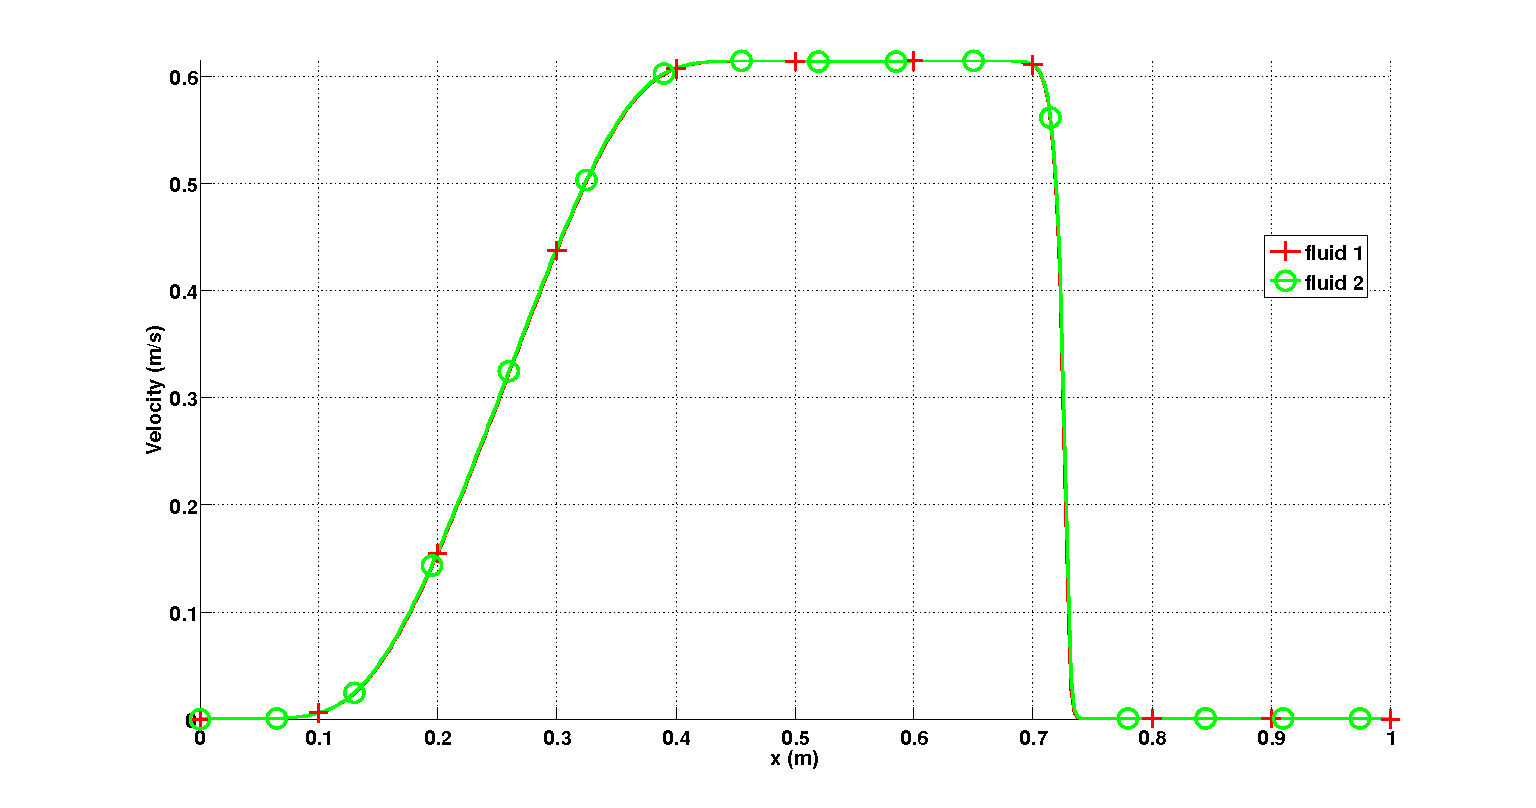
\includegraphics[width=\textwidth]{figures/relaxation_two_phases_velocity_fo_lf.png}
                \caption{Velocity}
                \label{fig:two-phase-vel}
        \end{subfigure}%
        \begin{subfigure}[b]{0.5\textwidth}
                \centering
                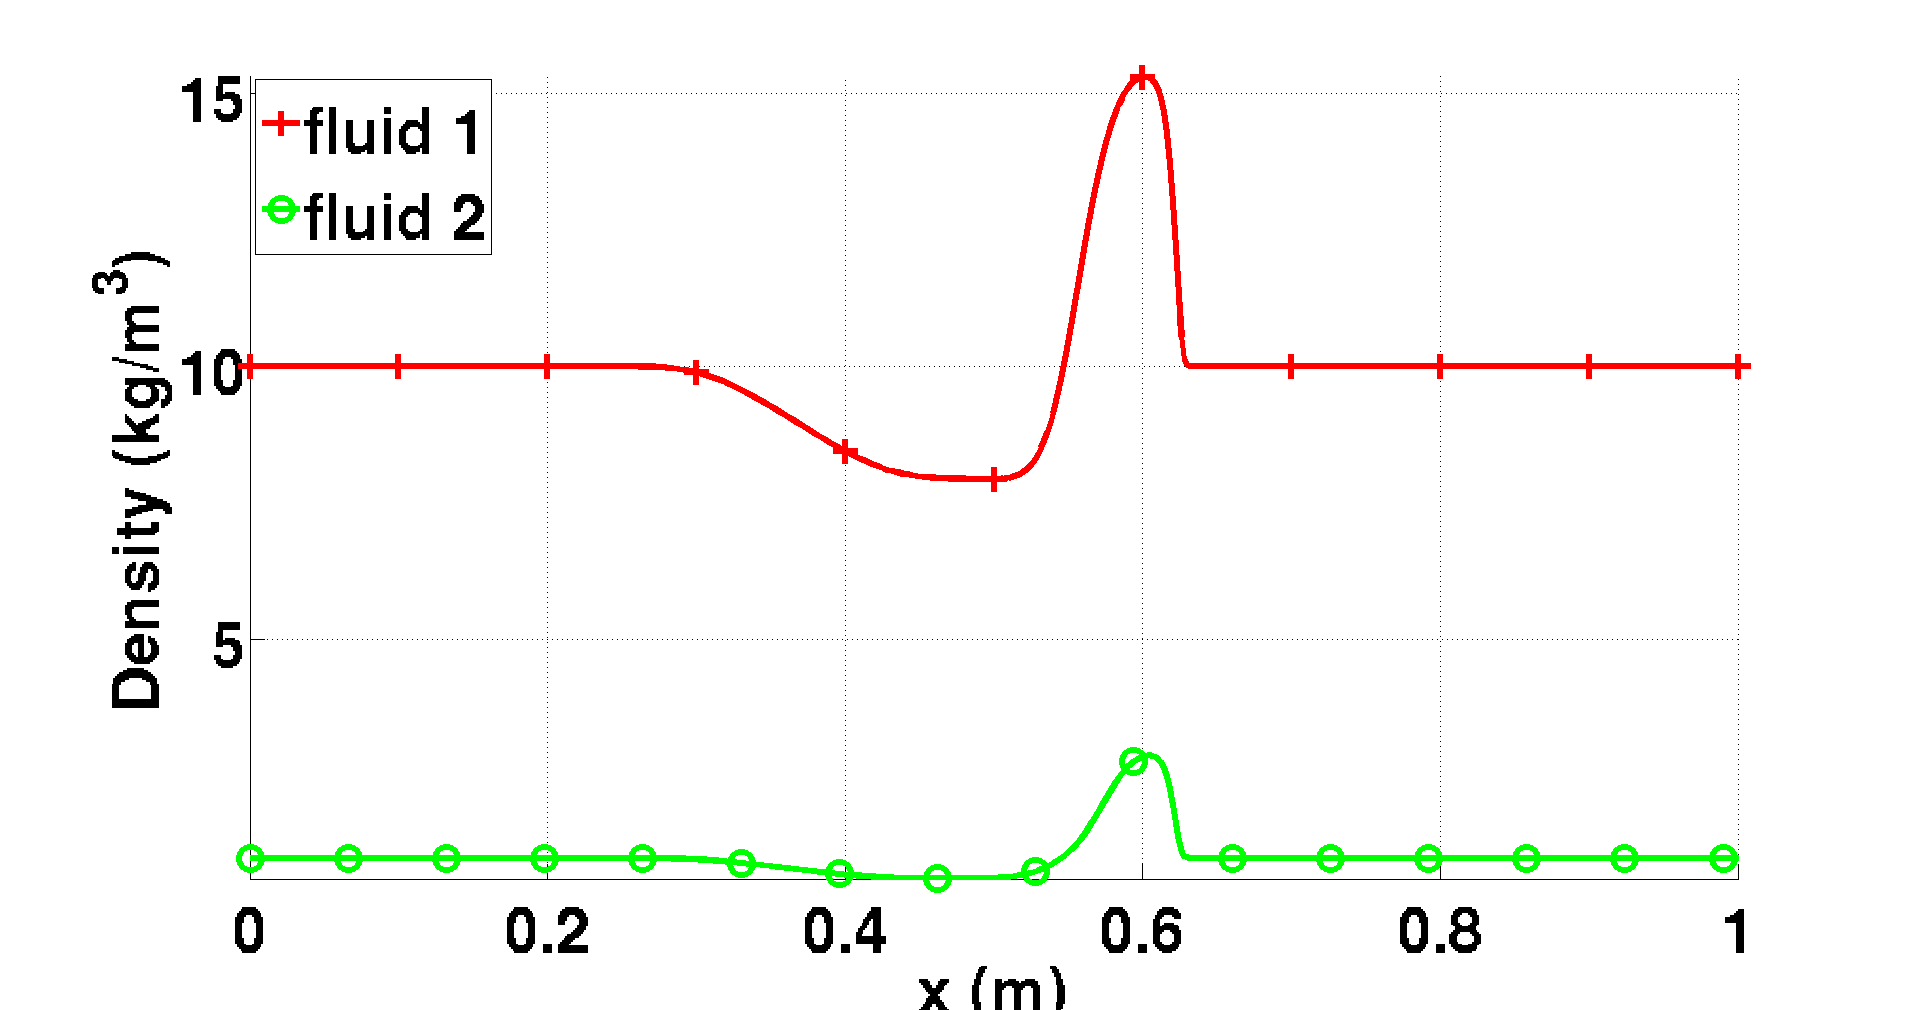
\includegraphics[width=\textwidth]{figures/relaxation_two_phases_density_fo_lf.png}
                \caption{Density}
                \label{fig:two-phase-density}
        \end{subfigure}
        
        \begin{subfigure}[b]{0.495\textwidth}
                \centering
                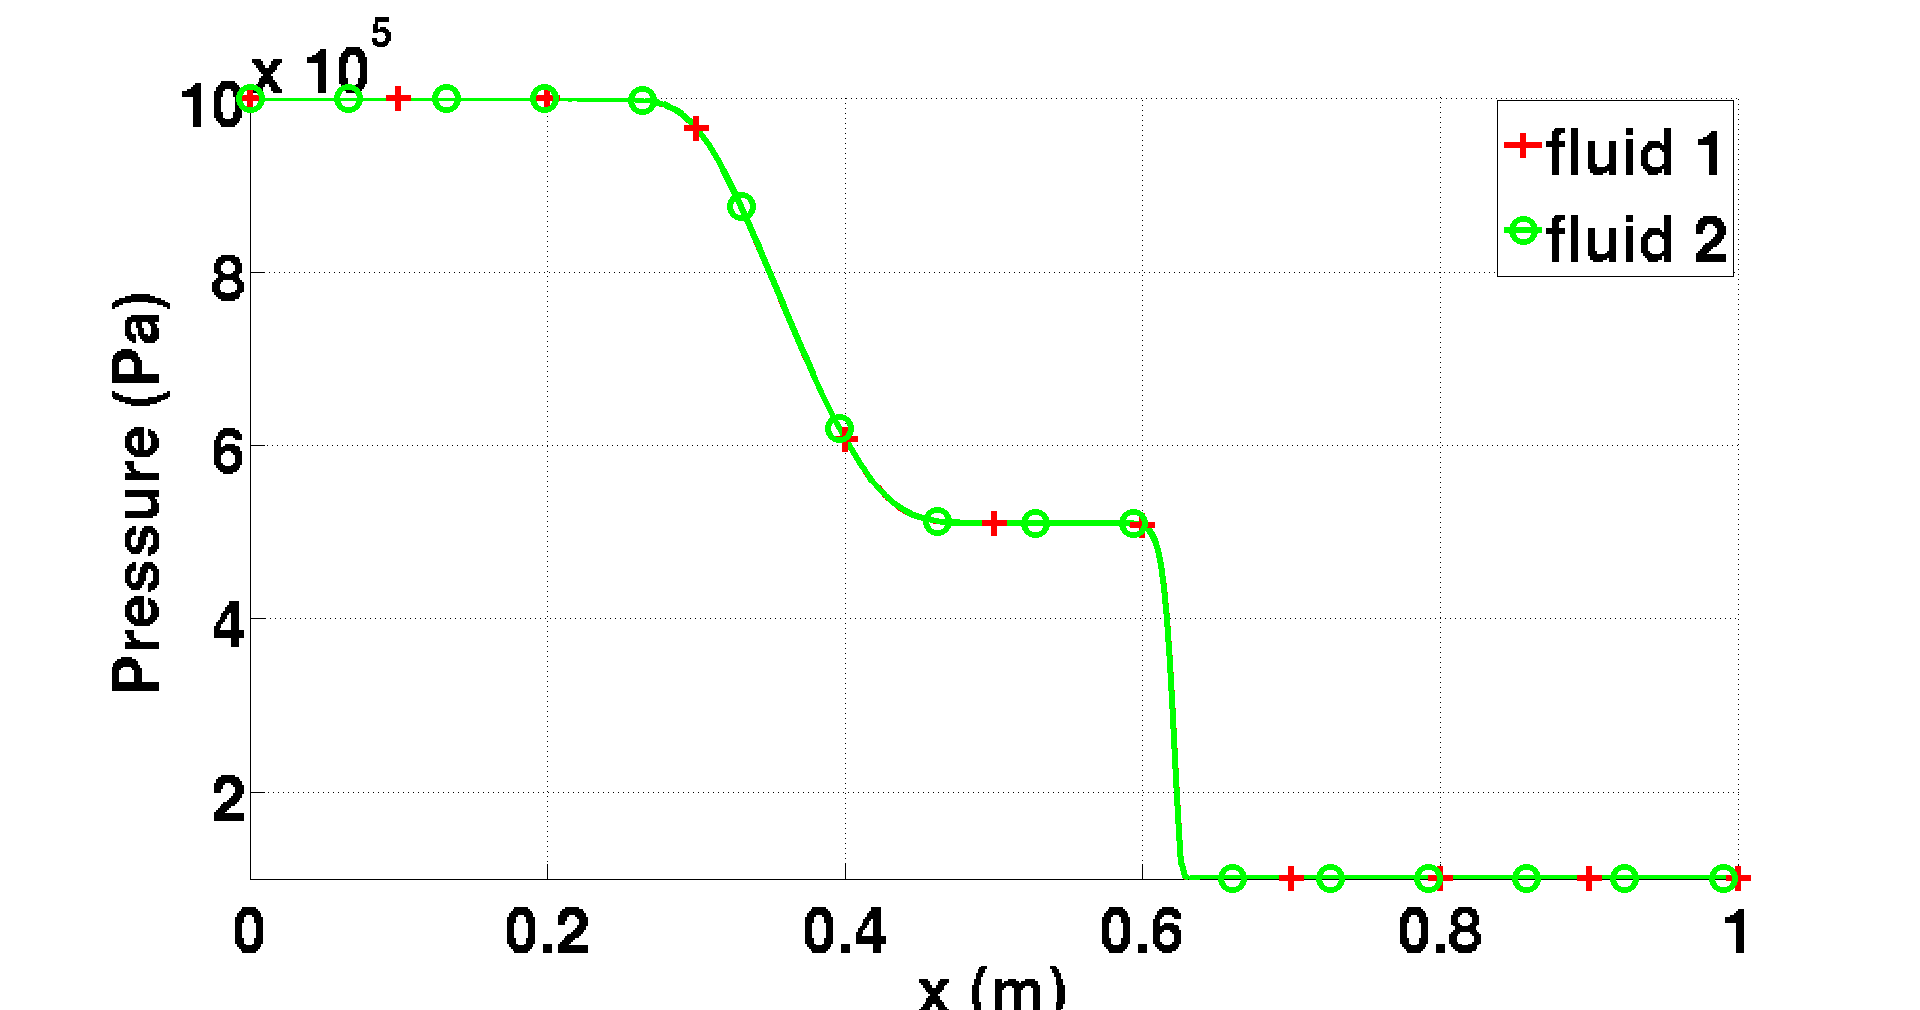
\includegraphics[width=\textwidth]{figures/relaxation_two_phases_pressure_fo_lf.png}
                \caption{Pressure}
                \label{fig:two-phase-press}
        \end{subfigure}        
        \begin{subfigure}[b]{0.495\textwidth}
                \centering
                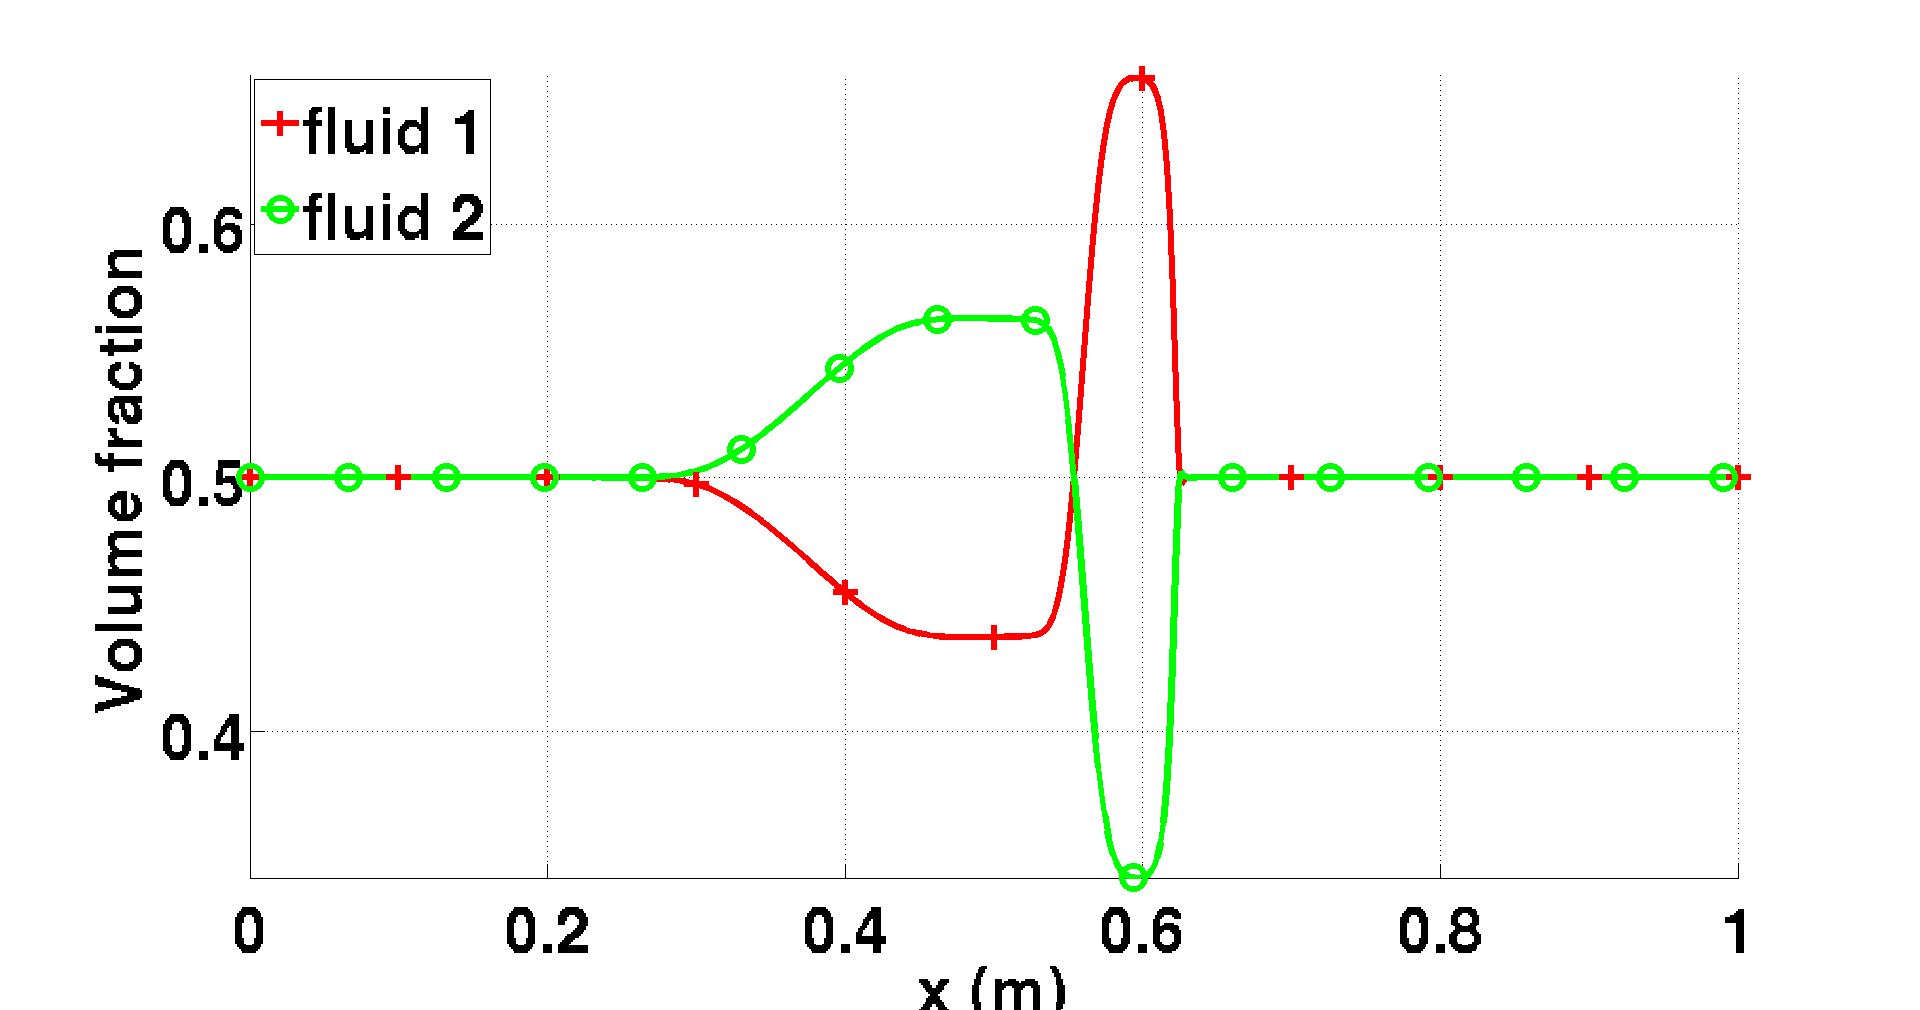
\includegraphics[width=\textwidth]{figures/relaxation_two_phases_volume_fraction_fo_lf.png}
                \caption{Volume fraction}
                \label{fig:two-phase-vf}
        \end{subfigure}
        \caption{Numerical solution of a two-phase flow with large relaxation coefficients at $t=0.18 \ s$.}\label{fig:two-phase}
\end{figure}
%
We further investigate the influence of the viscosity coefficients on the numerical solution by comparing several cases:
(1) all viscosity coefficients are equal (Lax-Friedrichs scheme already shown in \fig{fig:two-phase}), 
(2) the definitions for $\mu_k$ and $\kappa_k$ are unchanged but $\beta_k$ is set to zero (in doing so, we assess the effect of the viscous stabilization in the volume fraction equation), and 
(3) the viscosity coefficients $\kappa_k$ and $\beta_k$ are set to zero while $\mu_k$ is unchanged (in doing so, no stabilization is present in the continuity equations). For each case, density and volume fraction profiles are presented in \fig{fig:density} and \fig{fig:liq-vf}, respectively.
%
\begin{figure}[H]
        \centering
        \begin{subfigure}[b]{0.5\textwidth}
                \centering
                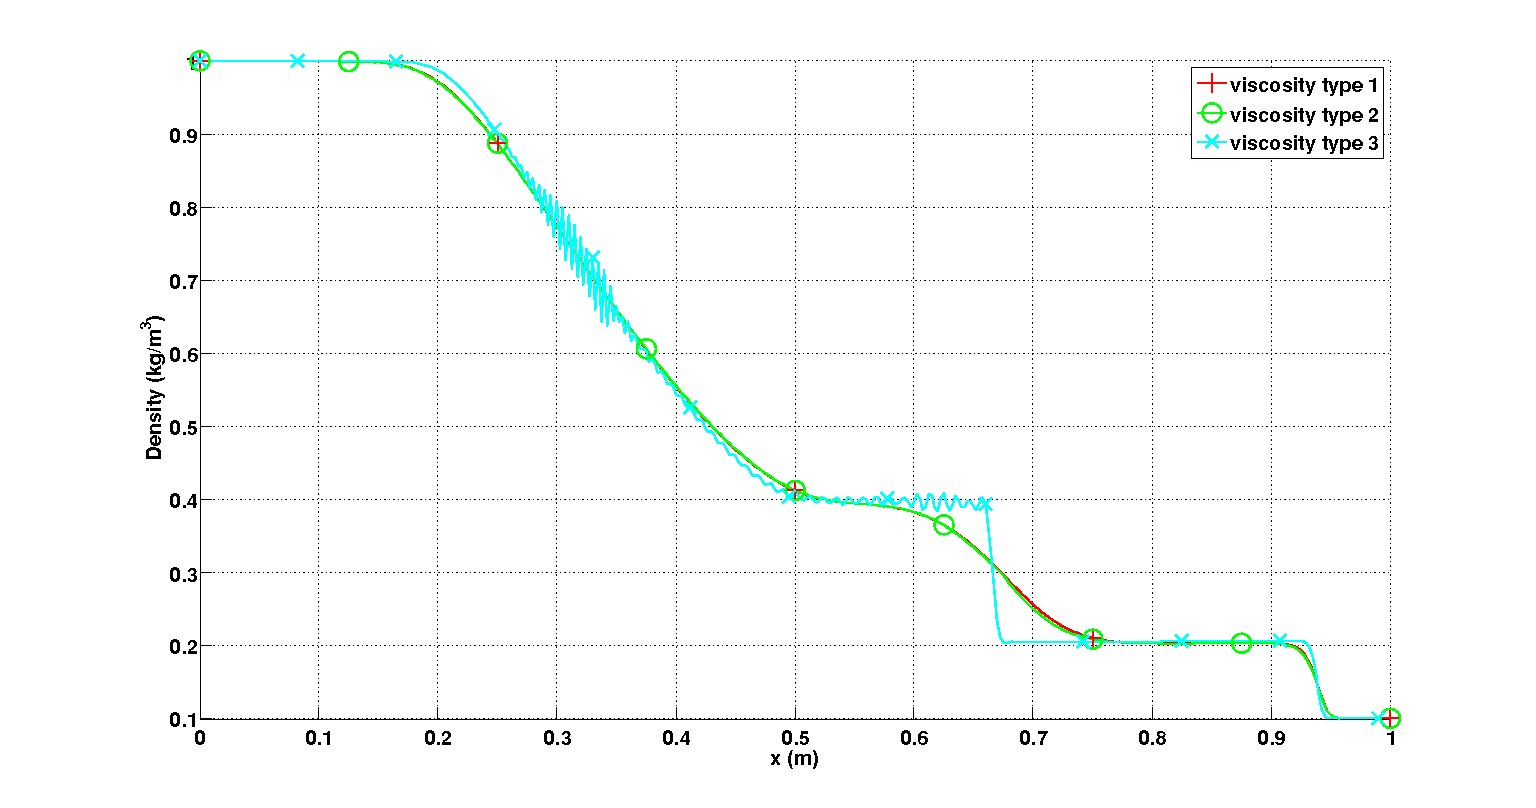
\includegraphics[width=\textwidth]{figures/relaxation_vapor_density_multiple_visc.png}
                \caption{Liquid density}
                \label{fig:liq-density}
        \end{subfigure}%
        \begin{subfigure}[b]{0.5\textwidth}
                \centering
                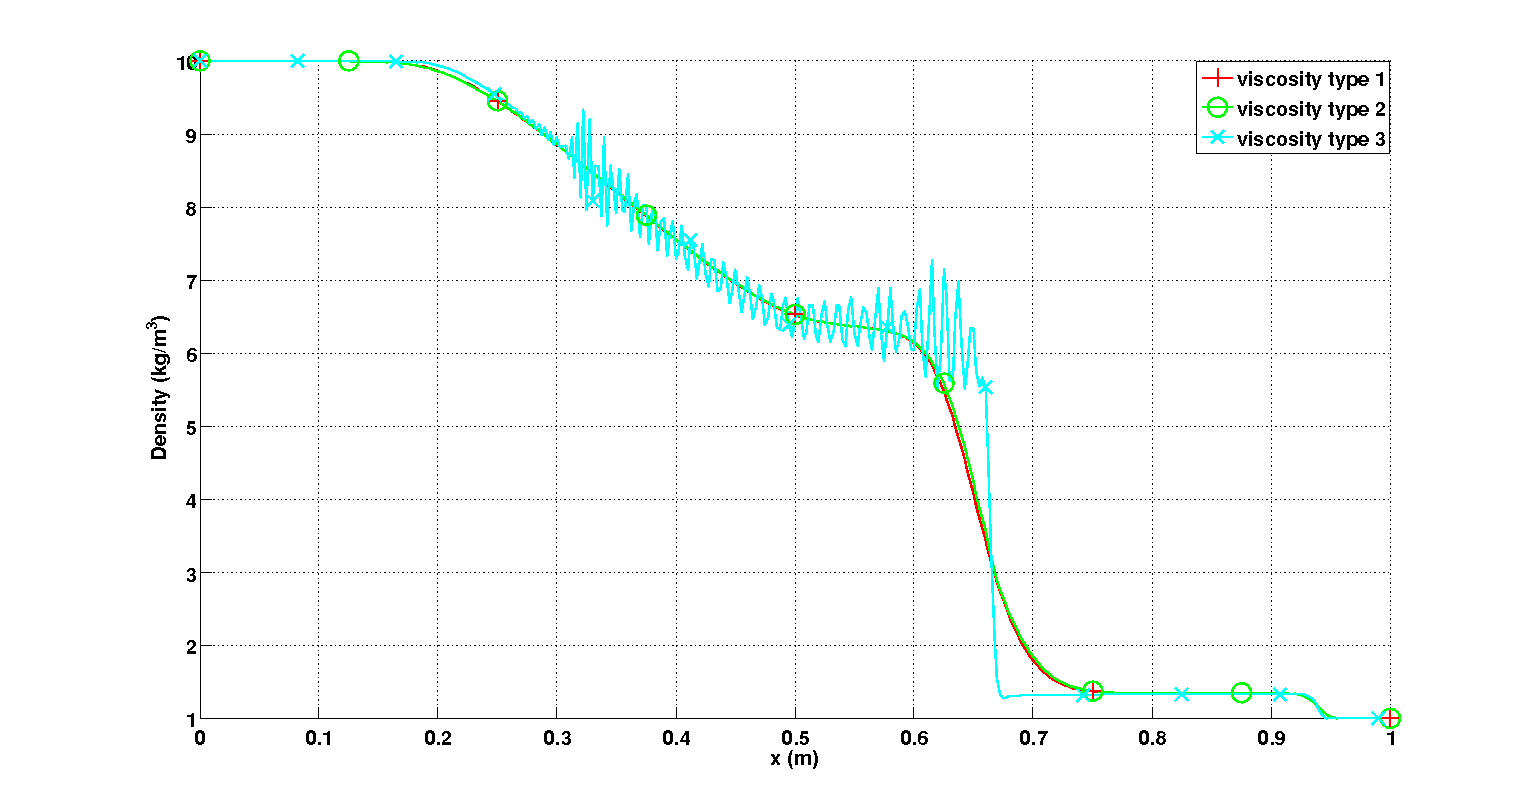
\includegraphics[width=\textwidth]{figures/relaxation_liquid_density_multiple_visc.png}
                \caption{Vapor density}
                \label{fig:vap-density}
        \end{subfigure}
        \caption{Numerical solutions of the liquid and vapor densities with large relaxation coefficients and three different viscosity types at $t=0.18 \ s$.}\label{fig:density}
\end{figure}
%
In cases (1) and (2), the numerical solutions do not display any instability in the density profiles. However, setting $\beta_k=0$ in case (2) results in spurious oscillations in the volume fraction profile near the contact region (see \fig{fig:liq-vf}). 
%
\begin{figure}[H]
        \centering
        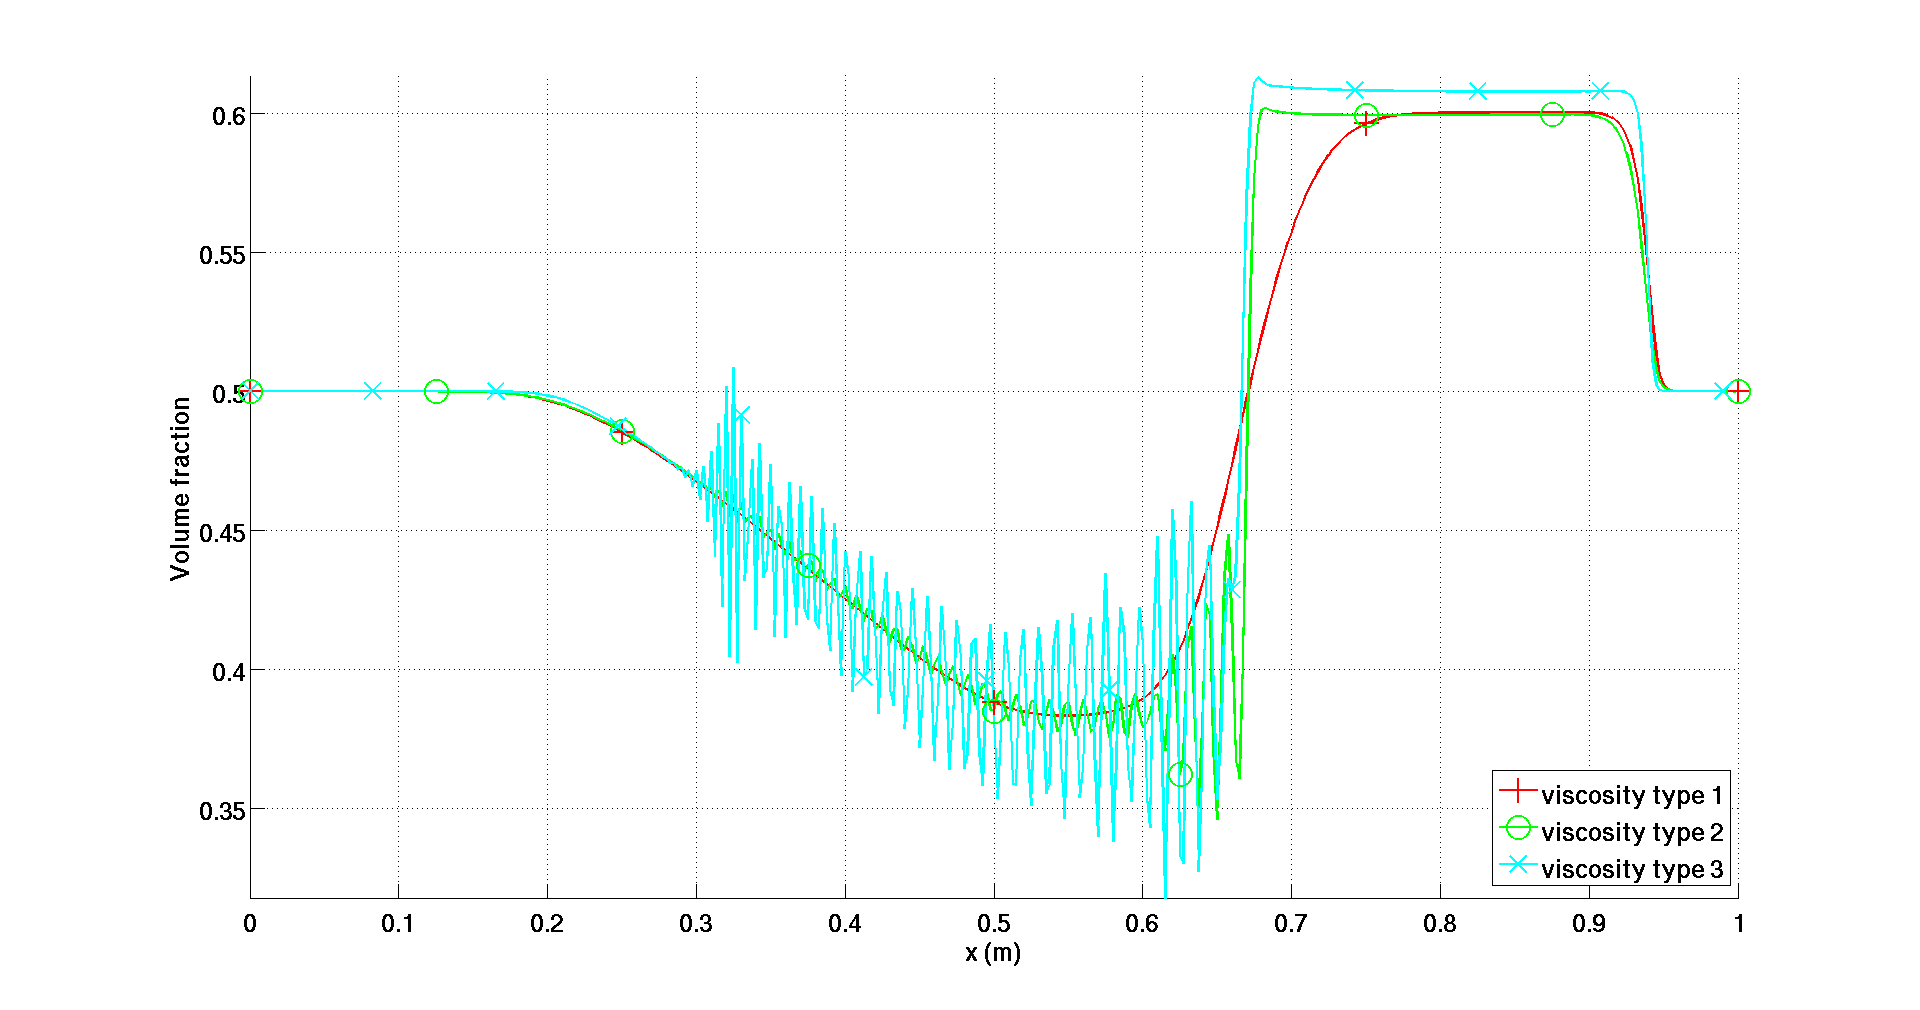
\includegraphics[width=\textwidth]{figures/relaxation_liquid_vf_multiple_visc.png}
        \caption{Liquid volume fraction}
        \label{fig:liq-vf}
\end{figure}
%
In the third case, the continuity and the volume fraction equations are no longer regularized since we have set $\kappa_k=\beta_k=0$; this leads to the formation of instabilities in the pre-contact region, the presence of an undershoot in the density profile and an overshoot in the volume fraction profile in the post-contact region as shown in \fig{fig:density} and \fig{fig:liq-vf}, respectively. This result is consistent with the study performed by Guermond et al. in \cite{jlg} for single-phase Euler equations where they compared numerical solutions obtained when employing a parabolic regularization (which included a dissipative term in the continuity equation) and the Navier-Stokes regularization.

We have also verified that if we set the relaxation coefficients $\mu_P$ and $\lambda_u$ to zero (which is equivalent to solving the Euler equations for each fluid independently), we recover 
the single-phase Euler shock tube results recently published in \cite{jlg1, jlg2, Marco_paper_low_mach} using the same viscous stabilization. 

%
%%%%%%%%%%%%%%%%%%%%%%%%%%%%%%%%%%%%%%%%%%%%%%%%%%%%%%%%%%%%%%%%%%%%%%%%%%%%%%%%%%%%%%%
\section{Conclusions}\label{sec:conclusion}
%%%%%%%%%%%%%%%%%%%%%%%%%%%%%%%%%%%%%%%%%%%%%%%%%%%%%%%%%%%%%%%%%%%%%%%%%%%%%%%%%%%%%%%
%%%%%%%%%%%%%%%%%%%%%%%%%%%%%%%%%%%%%%%%%%%%%%%%%%%%%%%%%%%%%%%%%%%%%%%%%%%%%
%
We have derived a viscous regularization for the hyperbolic Seven-Equation two-phase flow Model. The regularization ensures positivity of the entropy residual, 
uniqueness of the numerical solution for concave physical phasic entropy functions $s_k$, and is consistent with the viscous regularization derived for Euler equations 
when one of the phases disappears. 
We have also demonstrated that the proposed viscous regularization is compatible with the generalized Harten entropies that were initially derived for Euler equations. 

The viscous regularization for the SEM equations involves a set of two positive viscosity coefficients for each phase, $\mu_k$ and $\kappa_k$, and one for the volume fraction equation, $\beta_k$. 
The scaling of these viscosities is related to the numerical Reynolds and P\'eclet numbers, $\Re_k$, $\Pe_k^\mu$ and $\Pe_k^\kappa$. Adequate scaling of these numbers has been devised for two 
important cases: the low-Mach asymptotic limit and for non-isentropic flows. In the former case, we show that the incompressible equations are recovered when assuming that all of the non-dimensional 
numbers scale as one. The study of the non-isentropic case case shows that the scaling of the non-dimensionalized numbers is Mach-number dependent to ensure well-scaled dissipative terms in the vicinity of the shock.
Based on these results, adequate scaling of the viscosities can be obtained for all Mach numbers, as was the case for single-phase flows \cite{Marco_paper_low_mach}. 

We have also shown that the regularized SEM equations yields a regularized version of the five-equation flow model of Kapila by means of a Chapman-Enskog expansion.

The ability of the proposed regularization to stabilize the SEM equations was numerically demonstrated using a shock tube problem, with the definitions of the 
artificial viscosity coefficients borrowed from the Lax-Friedrichs scheme. We also analyzed the effect of removing stabilization from the volume fraction and the continuity equations.

As an extension of this work, the two-phase flow viscous regularization presented here should be utilized and tested with high-order, less dissipative, artificial viscosity schemes, 
such as the entropy viscosity method (e.g., see \cite{jlg1} for single-phase supersonic flows and \cite{Marco_paper_low_mach} single-phase subsonic and transonic flows). 
We also note that the proposed regularization can also be employed using definitions of viscosity coefficients traditionally used in two-phase flows, e.g., 
the Lapidus viscosity \cite{Lapidus_paper, Lapidus_book} and pressure-based viscosity for two-phase flows \cite{PBV_book}. We intend on reporting on these findings in a subsequent
publication. 

%
%%%%%%%%%%%%%%%%%%%%%%%%%%%%%%%%%%%%%%%%%%%%%%%%%%%%%%%%%%%%%%%%%%%%%%%%%%%%%
\bibliography{mybibfile}
%%%%%%%%%%%%%%%%%%%%%%%%%%%%%%%%%%%%%%%%%%%%%%%%%%%%%%%%%%%%%%%%%%%%%%%%%%%%%
\clearpage
%%%%%%%%%%%%%%%%%%%%%%%%%%%%%%%%%%%%%%%%%%%%%%%%%%%%%%%%%%%%%%%%%%%%%%%%%%%%%%
%%%%%%%%%%%%%%%%%%%%%%%%%%%%%%%%%%%%%%%%%%%%%%%%%%%
%
%  New template code for TAMU Theses and Dissertations starting Fall 2012.  
%  For more info about this template or the 
%  TAMU LaTeX User's Group, see http://www.howdy.me/.
%
%  Author: Wendy Lynn Turner 
%	 Version 1.0 
%  Last updated 8/5/2012
%
%%%%%%%%%%%%%%%%%%%%%%%%%%%%%%%%%%%%%%%%%%%%%%%%%%%

\begin{appendices}
%\titleformat{\chapter}{\centering\normalsize}{APPENDIX \thechapter}{0em}{\vskip .5\baselineskip\centering}
%\renewcommand{\appendixname}{APPENDIX}
%
%%%%%%%%%%%%%%%%%%%%%%%%%%%%%%%%%%%%%%%%%%%%%%%%%%%
%
%  New template code for TAMU Theses and Dissertations starting Fall 2012.  
%  For more info about this template or the 
%  TAMU LaTeX User's Group, see http://www.howdy.me/.
%
%  Author: Wendy Lynn Turner 
%	 Version 1.0 
%  Last updated 8/5/2012
%
%%%%%%%%%%%%%%%%%%%%%%%%%%%%%%%%%%%%%%%%%%%%%%%%%%%

%%%%%%%%%%%%%%%%%%%%%%%%%%%%%%%%%%%%%%%%%%%%%%%%%%%%%%%%%%%%%%%%%%%%%%
%%                           APPENDIX A 
%%%%%%%%%%%%%%%%%%%%%%%%%%%%%%%%%%%%%%%%%%%%%%%%%%%%%%%%%%%%%%%%%%%%%

\phantomsection

\section{Entropy equation for the multi-dimensional seven equation model without viscous regularization}\label{app:sev-equ-model-entropy}
%
This appendix provides the steps that lead to the derivation of the phasic entropy equation of the Seven-Equation two-phase flow Model \cite{SEM}. For the purpose of this appendix, two phases are considered with no interphase mass or heat transfer and denoted by the indexes $j$ and $k$. In the Seven-Equation two-phase flow Model, each phase obeys to the following set of equations (\eqt{eq:sev_equ-app}):
\begin{subequations}
\label{eq:sev_equ-app}
%
\begin{align}
\partial_t \left( \alpha_k  A\right) + A \mbold u_{int} \cdot \grad \alpha_k = A \mu_P \left( P_k - P_j \right) 
\end{align}
%
\begin{align}
\partial_t \left( \alpha_k \rho_k A \right) + \div \left( \alpha_k \rho_k \mbold u_k A \right) = 0 
\end{align}
%
\begin{multline}
\partial_t \left( \alpha_k \rho_k \mbold u_k A \right) + \div \left[ \alpha_k A \left( \rho_k \mbold u_k \otimes \mbold u_k + P_k \mathbb{I} \right) \right] =\\
\alpha_k P_k \grad A + P_{int} A \grad \alpha_k + A \lambda_u \left( \mbold u_j - \mbold u_k \right) 
\end{multline}
%
\begin{multline}
\partial_t \left( \alpha_k \rho_k E_k A \right) + \div \left[ \alpha_k A \mbold u_k \left( \rho_k E_k + P_k \right) \right] = \\
P_{int} A \mbold u_{int} \cdot \grad \alpha_k - A\mu_P \bar{P}_{int} \left( P_k-P_j \right) + \bar{\mbold u}_{int} A \lambda_u \left( \mbold u_j - \mbold u_k \right)
\end{multline}
\end{subequations}
where $\rho_k$, $\mbold u_k$, $E_k$ and $P_k$ denote the density, velocity, specific total energy, and pressure of  phase $k$, respectively. $\mu_P$ and $\lambda_u$ and the pressure and velocity relaxation parameters, respectively. We recall that we assume that the cross section $A$ is only function of space: $\partial_t A = 0$ (a value of $A \neq 1$ is mostly of practical important for 1D nozzle problems). 
Variables with subscript ${int}$ correspond to the interfacial variables; their definitions are given in \eqt{eq:sev_equ2-app}. 
\begin{equation}
\label{eq:sev_equ2-app}
\left\{
\begin{array}{lll}
P_{int} = \bar{P}_{int} - \frac{\grad \alpha_k}{|| \grad \alpha_k ||} \frac{Z_k Z_j}{Z_k + Z_j} \left( \mbold u_k-\mbold u_j \right) \\
\bar{P}_{int} = \frac{Z_k P_j + Z_j P_k}{Z_k + Z_j} \\
\mbold u_{int} = \bar{\mbold u}_{int} - \frac{\grad \alpha_k}{|| \grad \alpha_k ||} \frac{P_k - P_j}{Z_k + Z_j} \\
\bar{\mbold u}_{int} = \frac{Z_k \mbold u _k + Z_j \mbold u_j}{Z_k + Z_j}
\end{array}
\right.
\end{equation}
where $Z_k = \rho_k c_k$ and $Z_j = \rho_j c_j$ are the impedances of phases $k$ and $j$, respectively. The speed of sound is denoted by the symbol $c$. The sign function $sgn(x)$ returns $\pm 1$ according to the sign of variable $x$.

The first step in proving the entropy minimum principle for \eqt{eq:sev_equ-app} 
consists of recasting these equations using the primitive variables $(\alpha_k, \rho_k, \mbold u_k, e_k)$, where $e_k$ is the specific internal energy of phase $k$. We introduce the material derivative $\frac{D (\cdot)}{Dt} = \partial_t (\cdot) + \mbold u_k \cdot \grad (\cdot)$ for simplicity. 

The continuity equation can be expressed as follows:
\begin{equation}
\label{eq:cont1-app}
\alpha_k A \frac{D \rho_k}{Dt} + \rho_k A \mu_P \left( P_k-P_j \right) + \rho_k A \left( \mbold u_k-\mbold u_{int} \right) \cdot \grad \alpha_k + \rho_k \alpha_k \div \left( A \mbold u_k \right) = 0 \,.
\end{equation}
The momentum and continuity equations are combined to yield an equation for the velocity:
\begin{equation}
\label{eq:vel1-app}
\alpha_k \rho_k A \frac{D\mbold u_k}{Dt} + \grad \left( \alpha_k A P_k \right) = \alpha_k P_k \grad A + P_{int} A \grad \alpha_k + A \lambda_u \left( \mbold u_j-\mbold u_k \right) \,.
\end{equation}
A kinetic energy equation is obtained by multiplying the previous result by $\mbold u_k$ to yield:
\begin{multline}
\label{eq:kin1-app}
\alpha_k \rho_k A \frac{D\left(\mbold u_k^2/2\right)}{Dt} + \mbold u_k \grad \left( \alpha_k A P_k \right) = \\ \mbold u_k  \Big( \alpha_k P_k \grad A + P_{int} A \grad \alpha_k + A \lambda_u \left( \mbold u_j-\mbold u_k \right) \Big) \,.
\end{multline}
%
The internal energy equation is obtained by subtracting the above kinetic energy equation from the total energy equation:
\begin{multline}\label{eq:internal1}
\alpha_k \rho_k A \frac{D e_k}{Dt} + \alpha_k P_k \div \left(A \mbold u_k \right) = 
 P_{int} A \left(\mbold u_{int}-\mbold u_k \right) \cdot \grad \alpha_k \\
 - \bar{P}_{int} A \mu_P \left(P_k-P_j \right) + A \lambda_u \left(\mbold u_j-\mbold u_k  \right) \cdot \left(\bar{\mbold u}_{int}-\mbold u_k \right) \,.
\end{multline}

In the next step, we assume the existence of a phasic entropy $s_k$ that is function of the density $\rho_k$ and the  internal energy $e_k$. Using the chain rule, 
\begin{equation}
\frac{Ds_k}{Dt} = (s_\rho)_k \frac{D \rho_k}{Dt} + (s_e)_k \frac{De_k}{Dt},
\end{equation}
we combine the density and internal energy equations ($\rho_k (s_\rho)_k \times \eqt{eq:cont1-app}  + (s_e)_k \times \eqt{eq:internal1}$) to obtain  the following entropy equation :
\begin{multline}
\label{eq:ent1}
\alpha_k \rho_k A \frac{Ds_k}{Dt} + 
\underbrace{\alpha_k \left( P_k (s_e)_k + \rho_k^2 (s_\rho)_k \right)  \div \left( A \mbold u_k \right) }_\textrm{(a)} = \\
(s_e)_k A \left[ P_{int}(\mbold u_{int}-\mbold u_k)\cdot \grad \alpha_k - \bar{P}_{int} A \mu_P (P_k-P_j) + A \lambda_u (\bar{\mbold u}_{int}-\mbold u_k) \cdot (\mbold u_j-\mbold u_k)\right] \\
- \rho_k^2 (s_\rho)_k \left[ \mu_P A (P_k-P_j) + A(\mbold u_k-\mbold u_{int}) \cdot \grad \alpha_k\right] 
\end{multline}
where $(s_e)_k$ and $(s_\rho)_k$ denote the partial derivatives of entropy $s_k$ with respect to the internal energy $e_k$ and the density $\rho_k$, respectively.
The term denoted by (a) on the left-hand side of \eqt{eq:ent1} can be set to zero by invoking the second law of thermodynamics:
\begin{equation}
T_k ds_k = de_k - \frac{P_k}{\rho_k^2} d \rho_k \text{ with } (s_e)_k = \frac{1}{T_k} \text{ and } (s_\rho)_k = - \frac{P_k}{\rho_k^2} (s_e)_k
\end{equation}
which yields
\begin{equation}
\label{eq:ent2}
 P_k (s_e)_k + \rho_k^2 (s_\rho)_k = 0 .
\end{equation} 
% The above equation is equivalent to the application of the second law of thermodynamic law when assuming reversibility:

Finally,\eqt{eq:ent1} is as follows:
\begin{eqnarray}
\label{eq:ent3}
((s_e)_k)^{-1} \alpha_k \rho_k \frac{Ds_k}{Dt} = \underbrace{\left[ P_{int} (\mbold u_{int}-\mbold u_k) + P_k (\mbold u_k-\mbold u_{int}) \right] \cdot \grad \alpha_k}_\textrm{(b)} + \nonumber\\ 
\underbrace{\mu_P (P_k-P_j)(P_k-\bar{P}_{int})}_\textrm{(c)} + \underbrace{\lambda_u(\mbold u_j-\mbold u_k)\cdot(\bar{\mbold u}_{int}-\mbold u_k)}_\textrm{(d)}
\end{eqnarray}
The right-hand side of \eqt{eq:ent3} has been split into three terms, (b), (c), and (d); next we analyze each of these terms separately. The terms (c) and (d) can be easily recast by using the definitions of $\bar{\mbold u}_{int}$ and $\bar{P}_{int}$ given in \eqt{eq:sev_equ2-app}:
\begin{eqnarray}
\label{eq:ent4}
\mu_P (P_k-P_j)(P_k-\bar{P}_{int}) = \mu_P \frac{Z_k}{Z_k+Z_j} (P_j - P_k)^2\nonumber\\
\lambda_u(\mbold u_j-\mbold u_k)\cdot(\bar{\mbold u}_{int}-\mbold u_k) = \lambda_u \frac{Z_j}{Z_k+Z_j} (\mbold u_j - \mbold u_k)^2 
\end{eqnarray}
By definition, $\mu_P$, $\lambda_u$ and $Z_k$ are all positive. Thus, the above terms (c) and (d) are unconditionally positive. 

We now inspect term (b). Once again, we use the definitions of $P_{int}$ and $\mbold u_{int}$ and the following relations:
\begin{eqnarray}
\label{eq:ent4bis}
\mbold u_{int}-\mbold u_k &=& \frac{Z_j}{Z_k+Z_j}(\mbold u_j-\mbold u_k) -  \frac{\grad \alpha_k}{\| \grad \alpha_k \|} \frac{Pk-P_j}{Z_k+Z_j} \nonumber\\
P_{int}-P_k &=& \frac{Z_k}{Z_k+Z_j} (P_j-P_k) - \frac{\grad \alpha_k}{\| \grad \alpha_k \|} \frac{Z_k Z_j}{Z_k+Z_j} (\mbold u_k-\mbold u_j), \nonumber 
\end{eqnarray}
Then, term (b) becomes:
\begin{multline}
\label{eq:ent5}
\left[ P_{int} (\mbold u_{int}-\mbold u_k) + P_k (\mbold u_k-\mbold u_{int}) \right] \cdot \grad \alpha_k = (P_{int}-P_k)(\mbold u_{int}-\mbold u_k)\cdot \grad \alpha_k=   \\ 
\frac{Z_k}{\left( Z_k+Z_j \right)^2} \grad \alpha_k \cdot \left[ Z_j (\mbold u_j-\mbold u_k)(P_j-P_k)+\frac{\grad \alpha_k}{\| \grad \alpha_k \|} Z_j^2 (\mbold u_j-\mbold u_k)^2 \right. + \\ 
\left. \frac{\grad \alpha_k}{\| \grad \alpha_k \|}(P_k-P_j)^2 +  \frac{\grad \alpha_k \cdot \grad \alpha_k}{\| \grad \alpha_k \|^2}(P_k-P_j)Z_j (\mbold u_k-\mbold u_j) \right] 
\end{multline}
The above equation is factorized by $\|  \grad \alpha_k \|$ and then recast under a quadratic form using $\frac{\grad \alpha_k \cdot \grad \alpha_k}{\| \grad \alpha_k \|^2} = 1$. This yields:
\begin{align}
\label{eq:ent6}
\left[ (\mbold u_{int}-\mbold u_k)P_{int} + (\mbold u_k-\mbold u_{int})P_k \right] \grad \alpha_k &=  \nonumber \\
\| \grad \alpha_k \| \frac{Z_k }{\left( Z_k+Z_j \right)^2} \left[ Z_j (\mbold u_j-\mbold u_k) + \frac{\grad \alpha_k}{\| \grad \alpha_k \|}(P_k-P_j)\right]^2
\end{align}
Thus, using \eqt{eq:ent3}, \eqt{eq:ent4}, \eqt{eq:ent5} and \eqt{eq:ent6}, the entropy equation obtained in \cite{SEM} holds and is recalled here for convenience:
\begin{align}
(s_{e})_k^{-1} \alpha_k \rho_k A \frac{Ds_k}{Dt} &= \mu_P \frac{Z_k}{Z_k+Z_j} (P_j - P_k)^2 + \lambda_u \frac{Z_j}{Z_k+Z_j} (\mbold u_j -\mbold  u_k)^2 \nonumber
\\
& \| \grad \alpha_k \| \frac{Z_k}{\left( Z_k+Z_j \right)^2} \left[ Z_j (\mbold u_j-\mbold u_k)+\frac{\grad \alpha_k}{\| \grad \alpha_k \|}(P_k-P_j)\right]^2. \nonumber
\end{align}
%
\pagebreak{}
%%%%%%%%%%%%%%%%%%%%%%%%%%%%%%%%%%%%%%%%%%%%%%%%%%%
%
%  New template code for TAMU Theses and Dissertations starting Fall 2012.  
%  For more info about this template or the 
%  TAMU LaTeX User's Group, see http://www.howdy.me/.
%
%  Author: Wendy Lynn Turner 
%	 Version 1.0 
%  Last updated 8/5/2012
%
%%%%%%%%%%%%%%%%%%%%%%%%%%%%%%%%%%%%%%%%%%%%%%%%%%%

%%%%%%%%%%%%%%%%%%%%%%%%%%%%%%%%%%%%%%%%%%%%%%%%%%%%%%%%%%%%%%%%%%%%%%
%%                           APPENDIX B
%%%%%%%%%%%%%%%%%%%%%%%%%%%%%%%%%%%%%%%%%%%%%%%%%%%%%%%%%%%%%%%%%%%%%
%
\section{Compatibility of the viscous regularization for the seven-equation two-phase model with the generalized Harten entropies}\label{app:harden}
%
We investigate in this appendix whether the viscous regularization of the seven-equation two-phase model derived in \sct{sec:visc-regu} is compatible with some or all generalized entropies identified in Harten et al. \cite{Harten}. Considering the single-phase Euler equations, Harten et al. \cite{Harten} demonstrated that a function $\rho \mathscr{H}(s)$ is called a generalized entropy and is strictly concave if $\mathscr{H}$ is twice differential and
%
\begin{multline}\label{eq:generalized_ent}
\mathscr{H}' (s)  \geq 0, \ \ \ \ \mathscr{H}'(s)c_p^{-1} - \mathscr{H}'' \geq 0, \ \forall \left( \rho, e \right) \in \mathbb{R}_+^2 \ ,
\end{multline}
%
where $c_p \left( \rho, e \right) = T \partial_T s \left( \rho, e \right)$ is the specific heat at constant pressure ($T$ is a function of $e$ and $\rho$ through the equation of state). Because the seven-equation two-phase model was initially derived by assuming that each phase obeys the single-phase Euler equation, we want to investigate whether the above property still holds when considering the seven-equation model with viscous regularization included. To do so, we consider a phasic generalized entropy, $\mathscr{H}_k(s_k)$ and a phasic specific heat at constant pressure, $c_{p,k} \left( \rho_k, e_k \right) = T_k \partial_{T_k} s_k \left( \rho_k, T_k \right)$ characterized by \eqt{eq:generalized_ent}. The objective is to find an entropy inequality verified by $\rho_k \mathscr{H}_k(s_k)$.

We start from the entropy inequality verified by $s_k$, 
%
\begin{multline}\label{eq:ent-res-7-eqn-diss-terms-app}
\alpha_k \rho_k A \frac{Ds_k}{Dt} =  \mbold f_k \cdot \grad s_k + \div \left( \alpha_k A \rho_k \kappa_k  \grad s_k \right)  
- \alpha_k \rho_k A \kappa_k Q_k \\ + (s_e)_k \alpha_k A \rho_k \mu_k \grad^s \mbold u_k : \grad \mbold u_k.
\end{multline}
%
\eqt{eq:ent-res-7-eqn-diss-terms-app} is multiplied by $\mathscr{H}_k'(s_k)$ to yield:
%
\begin{multline}
\label{eq:ent-res-7-eqn-diss-terms-app2}
\alpha_k \rho_k A \frac{D\mathscr{H}_k(s_k)}{Dt} = \div \left( \alpha_k A \rho_k \kappa_k \grad \mathscr{H}_k (s_k) \right) - \mathscr{H}_k''(s_k) \alpha_k A \kappa_k \rho_k \| \grad s_k \|^2 + \\
\mathscr{H}_k'(s_k) \mbold f_k \cdot \grad s_k - \mathscr{H}_k'(s_k)\alpha_k \rho_k A \kappa_k Q_k +  \\
\mathscr{H}_k'(s_k)(s_e)_k \alpha_k A \rho_k \mu_k \grad^s \mbold u_k : \grad \mbold u_k 
\end{multline}
%
Let us now multiply the continuity equation of phase $k$ by $\mathscr{H}_k (s_k)$ and add the result to the above equation to obtain:
%
\begin{align}\label{eq:ent-res-7-eqn-diss-terms-app3}
\partial_t \left( \alpha_k \rho_k A \mathscr{H}_k(s_k)\right) + \div \left( \alpha_k \rho_k \mbold u_k A \mathscr{H}_k(s_k) \right)  &- \nonumber\\
\div \left[ \alpha_k A \rho_k \kappa_k \grad \mathscr{H}_k (s_k) + \alpha_k A \kappa_k \mathscr{H}_k (s_k) \grad \rho_k  \right. & \left. + A \kappa_k \rho_k \mathscr{H}_k (s_k) \grad \alpha_k\right] = \nonumber \\
\underbrace{-\mathscr{H}_k''(s_k) \alpha_k A \kappa_k \rho_k \| \grad s_k \|^2  - \mathscr{H}_k'(s_k) \alpha_k A \kappa_k \rho_k  Q_k}_{\mathbb{T}_0} &+\nonumber \\
\underbrace{ \mathscr{H}_k'(s_k)(s_e)_k  \alpha_k A \rho_k \mu_k \grad^s \mbold u_k : \grad \mbold u_k}_{\mathbb{T}_1} & .
\end{align}
%
As in \sct{sec:visc-regu}, the left-hand side of \eqt{eq:ent-res-7-eqn-diss-terms-app3} is split into two residuals denoted by $\mathbb{T}_0$ and $\mathbb{T}_1$ in order to study the sign of each of them. We start by studying the sign of $\mathbb{T}_1$ that is positive since it is assumed that $ \mathscr{H}_k'(s_k) \geq 0$. We now investigate the sign of $\mathbb{T}_0$. Using \eqt{eq:generalized_ent}, we have:
%
\begin{equation}\label{eq:new_quad_form}
- \mathbb{T}_0 \leq \mathscr{H}_k'(s_k) \alpha_k A \kappa_k \rho_k \left( c_{p,k}^{-1} \|\grad s_k\|^2 +  Q_k\right) \ .
\end{equation}
%
The right-hand side of \eqt{eq:new_quad_form} is a quadratic form that was already defined in Appendix 5 of \cite{jlg} and can be recast in the matrix form $X^t_k \mathbb{S} X_k$ where $\mathbb{S}$ is a $2 \times 2$ matrix and the vector $X_k$ was previously defined in \sct{sec:visc-regu}. In \cite{jlg}, matrix $\mathbb{S}$ is shown to be negative semi-definite which allows us to conclude that $\mathbb{T}_0$ is unconditionally positive using \eqt{eq:new_quad_form}. Then, knowing the sign of the two residuals $\mathbb{T}_0$ and $\mathbb{T}_1$, we conclude that:
%
\begin{align}\label{eq:ent-res-7-eqn-diss-terms-app4}
\partial_t \left( \alpha_k \rho_k A \mathscr{H}_k(s_k)\right) + \div \left( \alpha_k \rho_k \mbold u_k A \mathscr{H}_k(s_k) \right)  &- \nonumber\\
\div \left[ \alpha_k A \rho_k \kappa_k \grad \mathscr{H}_k (s_k) + \alpha_k A \kappa_k \mathscr{H}_k (s_k) \grad \rho_k  \right. & \left. + A \kappa_k \rho_k \mathscr{H}_k (s_k) \grad \alpha_k\right] \geq 0 \ .\nonumber 
\end{align}
%
For there, we conclude that an entropy inequality is satisfied for all generalized entropies $\rho_k \mathscr{H}_k (s_k)$ when using the viscous regularization derived in \sct{sec:visc-regu} for the seven-equation two-phase model. Note that the above inequality holds for the total entropy of the system as well, i.e., when summing over the phases (the source terms are determined from rational thermodynamics that requires summations over the phases).
%
\pagebreak{}
%
\end{appendices}
%%%%%%%%%%%%%%%%%%%%%%%%%%%%%%%%%%%%%%%%%%%%%%%%%%%%%%%%%%%%%%%%%%%%%%%%%%%%%%
\end{document}